\chapter{TINJAUAN PUSTAKA}
\label{chap:tinjauanpustaka}


\section{Hasil penelitian/perancangan terdahulu}
Dalam penelitian ini, penulis merujuk pada beberapa studi sebelumnya yang relevan. Penelitian-penelitian tersebut memiliki hubungan dengan topik yang sedang diteliti, sehingga dapat digunakan sebagai dasar untuk penelitian ini.

\subsection{\emph{Autonomous Thermal Vision Robotic System for Victims Recognition}}

Penelitian oleh Cruz Ulloa mengembangkan robot berkaki empat (\emph{quadruped-legged}) menggunakan Unitree A1 yang dilengkapi dengan kamera termal Optris Pi640. Robot ini dirancang untuk mendeteksi korban dalam misi pencarian dan penyelamatan di lingkungan pasca-bencana, dengan memanfaatkan citra termal yang dianalisis menggunakan algoritma \emph{Convolutional Neural Network (CNN)}. Hasil penelitian menunjukkan bahwa sistem ini mampu mencapai akurasi deteksi lebih dari 90\% dalam kondisi ekstrem, seperti lingkungan minim cahaya atau area yang dipenuhi puing bangunan. Robot ini beroperasi secara \emph{teleoperated} dan mampu menjelajah medan yang tidak rata, sehingga sangat membantu tim pencarian dalam menemukan korban yang terperangkap di lokasi bencana \cite{Cruz2021}. Sistem robot dibangun dengan menggunakan \emph{Robot Operating System (ROS) 1 Melodic}, seperti pada gambar \ref{fig:Quadruped dengan kamera termal untuk deteksi korban}

\begin{figure} [H] \centering
  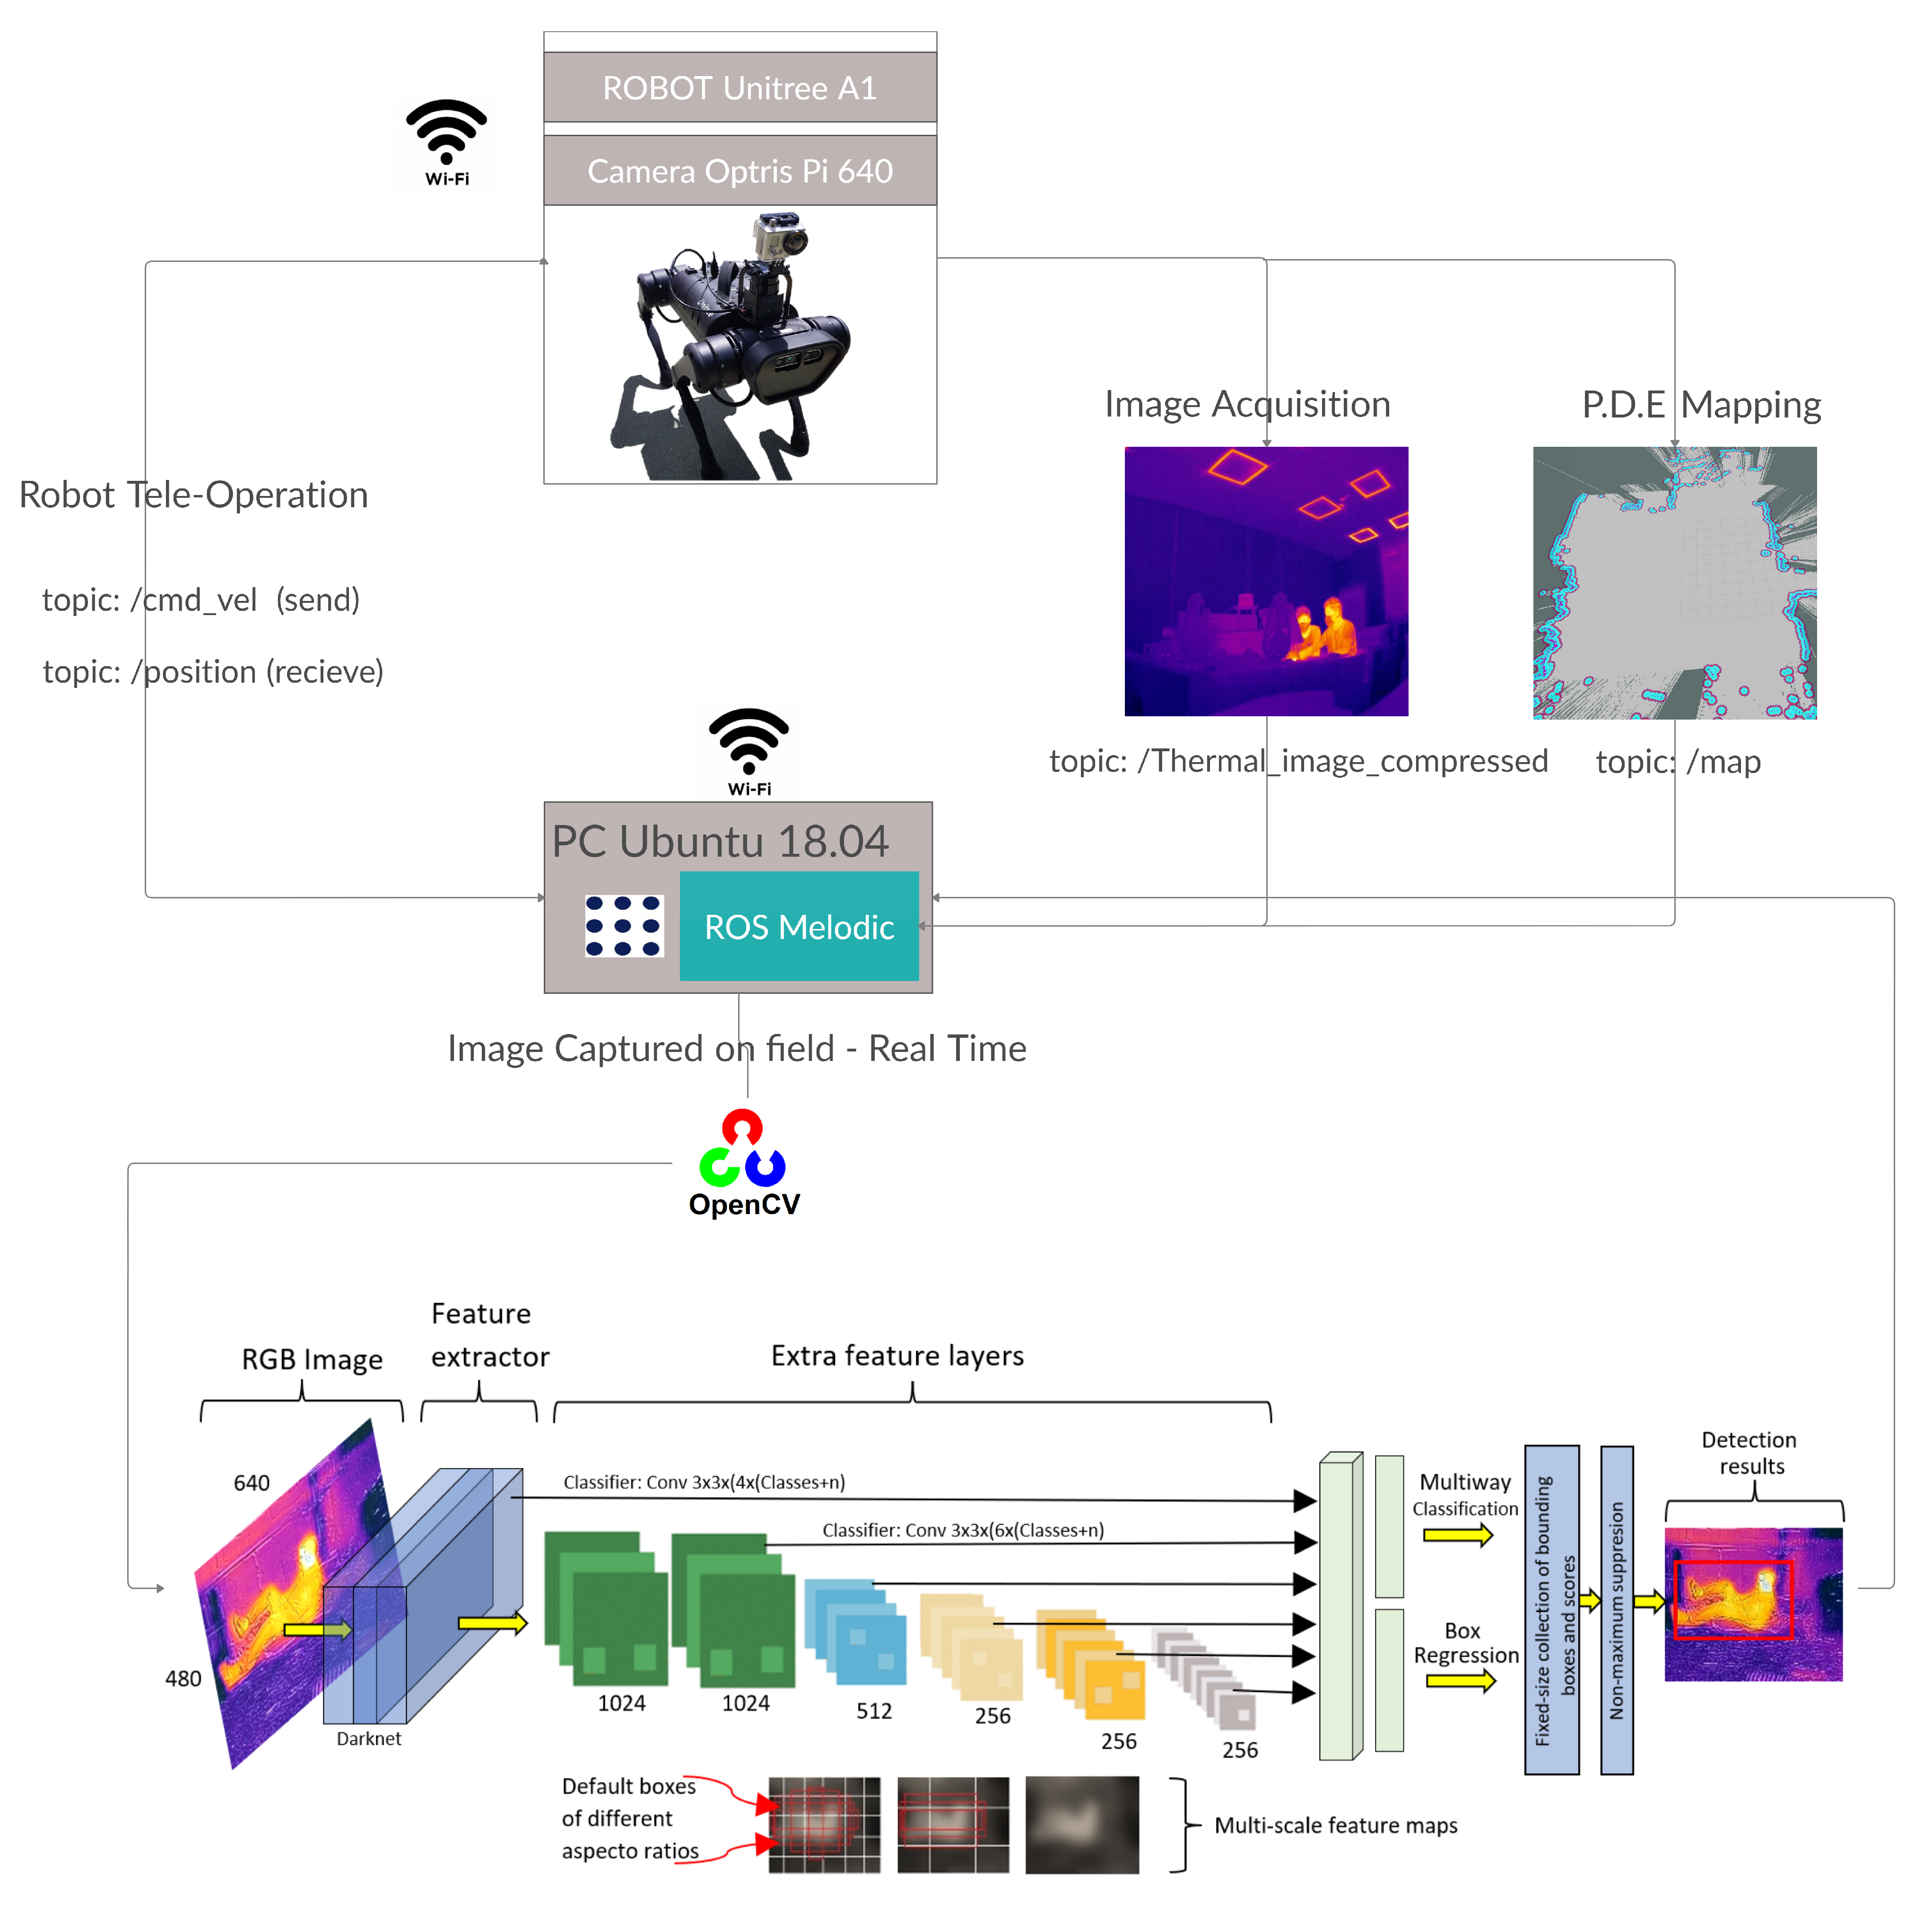
\includegraphics[scale=0.07]{gambar/bab2/unitreea1.png}
  \caption{Diagram sistem \emph{Autonomous Thermal Vision System for Victims Recognition} \cite{Cruz2021}}
  \label{fig:Quadruped  dengan kamera termal untuk deteksi korban}
\end{figure}

Gambar \ref{fig:Quadruped dengan kamera termal untuk deteksi korban}, terlihat bahwa robot ini dilengkapi dengan kamera termal yang terpasang pada bagian depan, yang digunakan untuk memantau dan mendeteksi objek atau korban dalam lingkungan sekitar. Gambar tersebut juga menunjukkan bagaimana data yang diperoleh dari kamera termal dikirim secara \emph{real-time} ke sistem komputer yang berjalan di atas PC dengan Ubuntu 18.04 dan \textit{ROS Melodic}, yang memproses dan mengklasifikasikan gambar menggunakan algoritma \textit{OpenCV} dan \textit{Convolutional Neural Networks (CNN)}. Proses ini memungkinkan robot untuk mengidentifikasi korban yang terdeteksi berdasarkan citra RGB termal dengan hasil \emph{detection result} berupa korban yang terdeteksi. Selain itu, robot ini juga dilengkapi dengan sistem pemetaan \textit{P.D.E} untuk meningkatkan akurasi deteksi serta perencanaan jalur dalam misi pencarian dan penyelamatan. Penelitian ini memiliki kesamaan dengan topik kami yang juga menggunakan robot berkaki empat dan kamera termal untuk mendeteksi objek. Namun, fokus penelitian ini adalah pada misi pencarian dan penyelamatan, sedangkan penelitian kami berfokus pada pemantauan komponen gardu listrik.

\subsection{\emph{Image Processing Technique Applied to Electrical
Substations Based on Drones With Thermal Vision
for Predictive Maintenance}}
Penelitian ini mengusulkan penggunaan \emph{VANT} \emph{(Vehículo Aéreo No Tripulado)} atau drone, yang dilengkapi dengan dua jenis kamera: \emph{kamera tradisional} untuk menangkap gambar visual dan \emph{thermal camera} untuk memperoleh gambar inframerah yang dapat menunjukkan suhu komponen di gardu induk. Drone ini dilengkapi dengan sistem navigasi dan pengendalian yang memungkinkan operasi otonom di sekitar gardu induk. Data gambar yang diambil oleh drone diproses menggunakan teknik \emph{image processing} untuk mengidentifikasi \emph{hot spots} atau titik panas pada komponen gardu induk.

\begin{figure}[H]
  \centering
  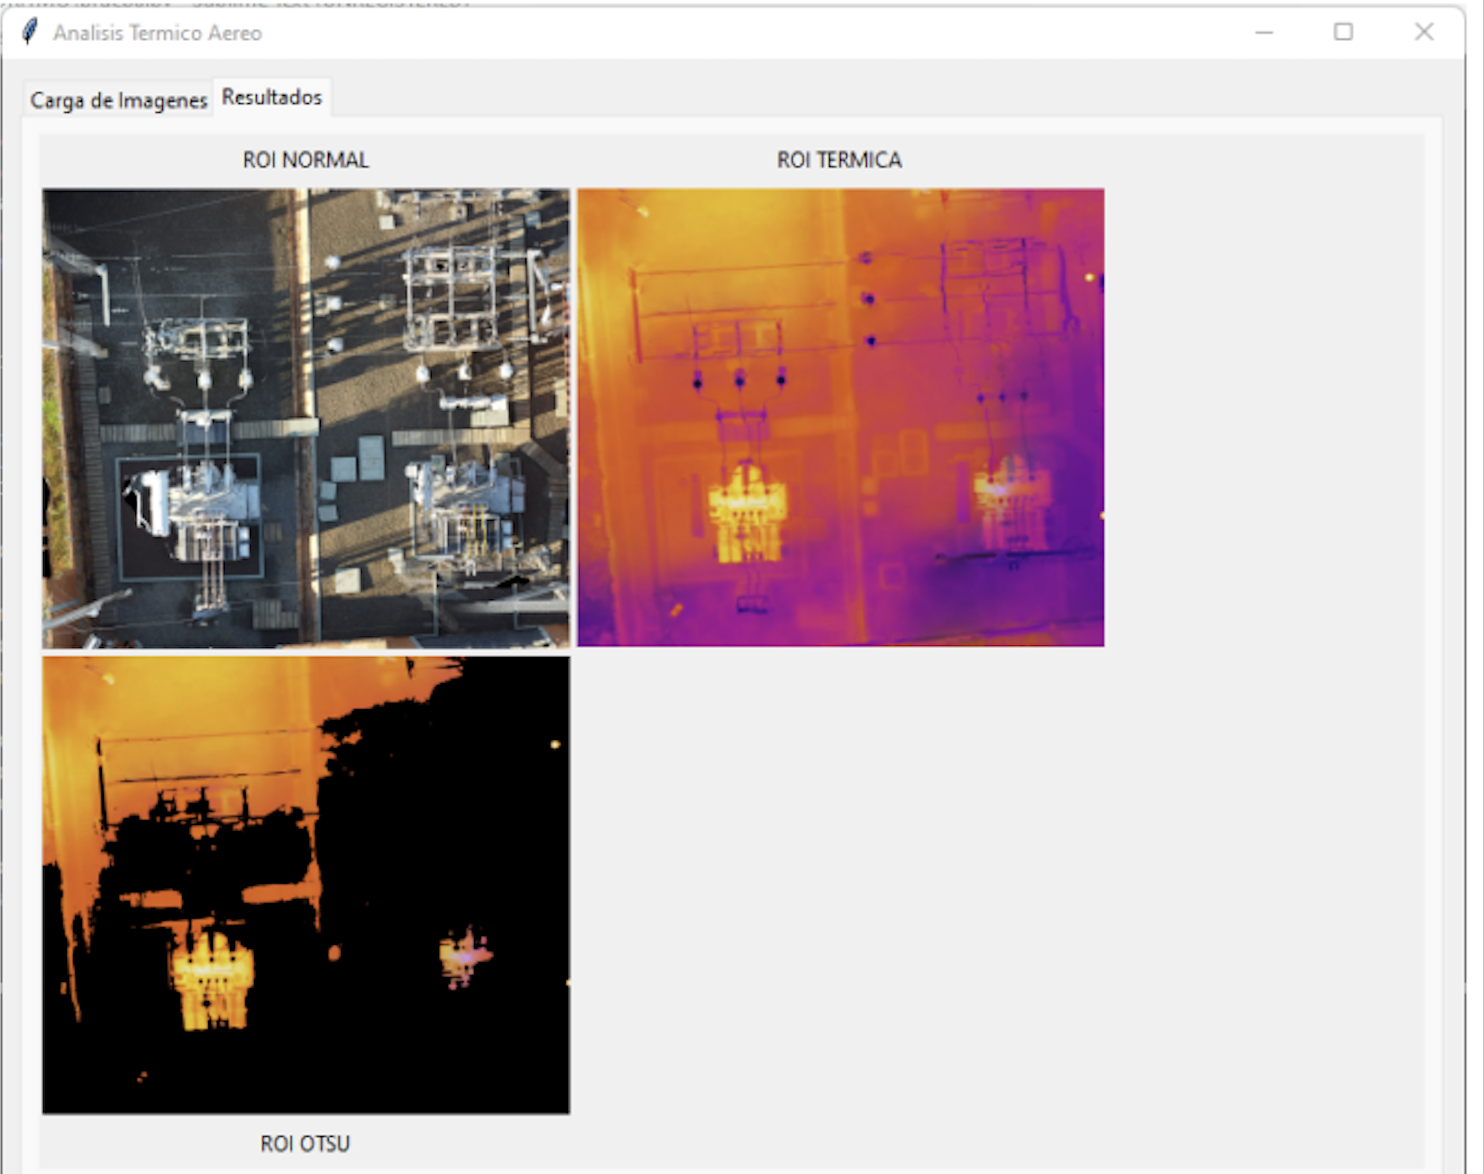
\includegraphics[scale=0.34]{gambar/bab2/drone.png}
  \caption{\emph{GUI} Drone dengan kamera termal untuk pemantauan gardu induk.}
  \label{fig:Drone dengan kamera termal untuk pemantauan gardu induk}
\end{figure}

Gambar \ref{fig:Drone dengan kamera termal untuk pemantauan gardu induk} menunjukkan antarmuka grafis pengguna (\emph{GUI}) yang digunakan untuk memproses dan menganalisis gambar termal yang diambil oleh drone. Pada gambar tersebut, terdapat tiga jenis gambar yang ditampilkan. Gambar pertama, yaitu gambar normal di sisi kiri atas, menunjukkan tampilan visual dari area gardu induk yang dipilih. Gambar ini memberikan gambaran umum tentang struktur gardu induk secara keseluruhan. Di sisi kanan atas, gambar termal menampilkan suhu komponen gardu induk dalam bentuk warna yang berbeda, di mana warna yang lebih terang menunjukkan suhu yang lebih tinggi, yang mengindikasikan adanya perbedaan suhu pada komponen tersebut. Gambar ini memungkinkan deteksi titik panas yang berpotensi menjadi masalah.  Di bagian bawah gambar, terlihat gambar hasil pemrosesan yang telah dianalisis menggunakan teknik \emph{image processing}. Gambar ini menunjukkan area yang telah diproses untuk mendeteksi titik panas pada komponen gardu induk. Teknik segmentasi \emph{OTSU} digunakan untuk memisahkan area dengan suhu tinggi, yang dapat menunjukkan potensi masalah seperti \emph{overheat} pada komponen gardu induk. Dengan demikian, gambar hasil pemrosesan memberikan informasi yang lebih terfokus mengenai area yang membutuhkan perhatian lebih dalam pemeliharaan. Hasil analisis ini dapat digunakan untuk memprediksi potensi kerusakan pada komponen dan mengambil tindakan pencegahan yang diperlukan. Penelitian ini menunjukkan bahwa penggunaan drone dengan kamera termal dapat meningkatkan efisiensi dan akurasi dalam pemantauan gardu induk, serta meminimalkan risiko keselamatan bagi petugas yang harus melakukan inspeksi langsung di lokasi gardu \cite{Prieto2022}. Penelitian ini memiliki kesamaan dengan topik kami yang juga menggunakan kamera termal untuk pemantauan komponen gardu listrik.



\section{Teori/Konsep Dasar}
Subbab ini membahas berbagai teori dan konsep dasar yang menjadi landasan dalam penyusunan tugas akhir. Penjelasan dalam bab ini mencakup berbagai teori yang relevan dan digunakan dalam pelaksanaan penelitian.

\subsection{Gardu Listrik}
\sloppy
Gardu listrik merupakan salah satu komponen vital dalam sistem kelistrikan yang berfungsi sebagai titik penghubung antara pembangkit listrik dan jaringan distribusi. Melalui gardu listrik, aliran energi listrik dapat diatur dan dialirkan secara efisien dari sumber pembangkit menuju konsumen akhir \cite{stevenson1994power}. Proses transmisi dan distribusi energi listrik tidak dapat dilakukan secara aman dan terkontrol tanpa adanya gardu listrik. Secara umum, terdapat beberapa jenis gardu listrik, antara lain gardu induk dan gardu pembangkit. Gardu induk memiliki fungsi utama untuk menurunkan tegangan listrik dari tingkat tinggi, yang digunakan dalam proses transmisi, menjadi tegangan menengah atau rendah agar aman untuk digunakan oleh konsumen. Gardu ini umumnya terletak di antara pembangkit dan kawasan konsumen, baik permukiman maupun kawasan industri. Sementara itu, gardu pembangkit merupakan fasilitas yang berada di dekat sumber energi primer, seperti pembangkit listrik tenaga air (PLTA), pembangkit listrik tenaga uap (PLTU), atau jenis pembangkit lainnya. Gardu ini berfungsi untuk menyalurkan energi listrik yang dihasilkan dari proses konversi energi primer ke jaringan transmisi. Untuk mendukung fungsinya, gardu listrik dilengkapi dengan berbagai peralatan kelistrikan, seperti transformator, pemutus sirkuit, isolator, dan komponen lainya untuk menjamin keandalan sistem. Keandalan gardu listrik sangat berpengaruh terhadap kualitas dan kontinuitas pasokan energi listrik \cite{gonen2016electric}.

\subsubsection{2.2.1.1 Gardu Induk}
Gardu induk merupakan salah satu komponen vital dalam sistem tenaga listrik yang berfungsi untuk mengubah, mengatur, dan menyalurkan energi listrik dari pembangkit ke konsumen melalui jaringan transmisi dan distribusi. Fungsi gardu mencakup menaikkan tegangan listrik dari pembangkit untuk keperluan transmisi jarak jauh, serta menurunkan tegangan sebelum didistribusikan ke konsumen akhir. Tegangan tinggi diperlukan dalam proses transmisi untuk meminimalkan rugi-rugi daya (\emph{losses}) yang terjadi akibat resistansi saluran, sementara penurunan tegangan dibutuhkan agar sesuai dengan batasan keamanan dan kebutuhan perangkat di sisi konsumen. Berdasarkan tingkat tegangan yang diolah, gardu induk diklasifikasikan menjadi beberapa jenis utama, yaitu gardu induk tegangan ekstra tinggi (GITET), gardu induk tegangan tinggi (GIT), gardu induk tegangan menengah (GIM), dan gardu induk tegangan rendah (GIR). GITET beroperasi pada tegangan di atas 500 kilovolt (kV) dan digunakan untuk transmisi daya dalam skala besar antarpulau atau antardaerah beban yang berjauhan, karena efisiensinya dalam mengurangi kehilangan daya selama proses transmisi. GIT menangani tegangan pada rentang 150--500 kV, berfungsi sebagai titik interkoneksi antar sistem transmisi serta sebagai tempat pengaturan pembebanan antara pembangkit dan jaringan utama. Selanjutnya, GIM beroperasi pada tegangan menengah antara 20--150 kV, dan biasanya digunakan untuk menghubungkan sistem transmisi ke jaringan distribusi, baik di wilayah industri maupun kawasan pemukiman padat. Terakhir, GIR mengelola tegangan di bawah 20 kV, dan bertugas menyuplai energi listrik langsung ke konsumen akhir seperti rumah tangga, pertokoan, dan industri kecil.

Secara umum, setiap gardu induk dilengkapi dengan berbagai peralatan kelistrikan utama, seperti transformator daya untuk konversi tegangan, pemutus sirkuit (\emph{circuit breaker}) untuk proteksi dan pemisahan rangkaian, isolator untuk pemisahan fisik komponen bertegangan, serta perangkat pengukuran dan kontrol lainnya. Selain itu, gardu induk juga dilengkapi dengan sistem proteksi otomatis untuk mendeteksi gangguan dan mencegah kerusakan pada peralatan. Keandalan dan efisiensi operasional gardu induk sangat menentukan kestabilan sistem tenaga listrik secara keseluruhan, terutama dalam menghadapi fluktuasi beban, kondisi darurat, maupun pemeliharaan jaringan\cite{gonen2016electric}.



\subsubsection{2.2.1.2 Transformator}

Transformator merupakan salah satu komponen utama dalam gardu listrik yang berfungsi untuk mengubah tingkat tegangan sesuai kebutuhan dalam proses transmisi maupun distribusi energi listrik. Transformator bekerja berdasarkan prinsip induksi elektromagnetik, di mana energi listrik dialirkan melalui dua kumparan yang terpisah secara galvanis namun terhubung melalui inti magnetik. Dalam sistem tenaga listrik, transformator tidak hanya digunakan untuk mengatur level tegangan, tetapi juga untuk meningkatkan efisiensi dan keamanan sistem. Salah satu jenis transformator yang umum digunakan pada gardu listrik adalah transformator daya. Transformator ini berfungsi untuk menyesuaikan tegangan agar sesuai dengan kebutuhan sistem, serta meminimalkan rugi-rugi daya selama proses transmisi jarak jauh. Berdasarkan fungsinya, transformator daya dibedakan menjadi dua jenis utama, yaitu transformator \emph{step-up} dan transformator \emph{step-down}. Transformator \emph{step-up} digunakan di sisi pembangkit untuk menaikkan tegangan listrik ke tingkat yang lebih tinggi agar proses transmisi menjadi lebih efisien dan rugi daya dapat dikurangi. Sebaliknya, transformator \emph{step-down} digunakan di sisi distribusi untuk menurunkan tegangan ke tingkat yang lebih rendah agar aman digunakan oleh konsumen akhir, seperti rumah tangga dan industri.

Selain transformator daya, gardu listrik juga dilengkapi dengan transformator arus atau \emph{current transformer (CT)}. \emph{CT} berfungsi untuk mengubah arus listrik yang besar pada sistem tenaga menjadi arus yang lebih kecil dan aman untuk keperluan pengukuran, pengendalian, dan proteksi. Dengan menggunakan \emph{CT}, perangkat seperti relai proteksi, sistem pemantauan, dan peralatan metering dapat mengamati kondisi arus tanpa harus langsung berhubungan dengan arus utama yang tinggi dan berbahaya. Transformator arus dirancang dengan akurasi dan rasio transformasi tertentu untuk memastikan bahwa sinyal arus yang dikirimkan ke peralatan sekunder tetap mencerminkan kondisi nyata sistem. Dari sisi termal, transformator daya umumnya dirancang untuk beroperasi pada suhu maksimum antara 105\textdegree{}C hingga 110\textdegree{}C, tergantung pada kelas isolasi termalnya, seperti kelas A (105\textdegree{}C), B (130\textdegree{}C), atau F (155\textdegree{}C). Sementara itu, transformator arus (CT) biasanya dirancang untuk beroperasi pada rentang suhu antara 70\textdegree{}C hingga 90\textdegree{}C, tergantung pada standar pabrikan dan klasifikasi aplikasinya. Meskipun arus yang masuk ke \emph{CT} merupakan arus tinggi, arus keluarannya kecil sehingga beban termal yang diterima relatif rendah. Namun demikian, \emph{CT} tetap memerlukan sistem ventilasi atau pendinginan yang memadai agar kinerja pengukuran tetap stabil dan umur operasional peralatan dapat terjaga. Pengelolaan suhu operasional yang baik pada kedua jenis transformator ini menjadi faktor krusial untuk menjaga keandalan dan efisiensi sistem tenaga secara keseluruhan \cite{stevenson1994power}.


\subsubsection{2.2.1.3 Pemutus Sirkuit (\emph{Circuit Breaker})}
Pemutus sirkuit adalah perangkat yang berfungsi untuk melindungi sistem kelistrikan dari arus lebih (\emph{overcurrent}) dan hubung singkat (\emph{short circuit}). Pemutus sirkuit dapat secara otomatis memutuskan aliran listrik ketika terdeteksi adanya gangguan, sehingga mencegah kerusakan pada peralatan dan menjaga keselamatan sistem. Terdapat berbagai jenis pemutus sirkuit, termasuk pemutus sirkuit otomatis (\emph{automatic circuit breaker}) dan pemutus sirkuit manual (\emph{manual circuit breaker}), yang masing-masing memiliki aplikasi dan karakteristik yang berbeda Pemeliharaan dan pengujian berkala terhadap pemutus sirkuit sangat penting untuk memastikan bahwa perangkat ini berfungsi dengan baik saat dibutuhkan. Suhu operasi pemutus sirkuit biasanya berkisar antara -25\textdegree{}C hingga 55\textdegree{}C, dan overheating dapat terjadi jika suhu melebihi 85\textdegree{}C, yang dapat menyebabkan kerusakan pada mekanisme pemutus \cite{Ilomets2020}.


\subsubsection{2.2.1.4 \emph{Arrester}}
\emph{Arrester}, atau \emph{lightning arrester}, merupakan perangkat pelindung dalam sistem kelistrikan yang berfungsi untuk mengamankan peralatan dari lonjakan tegangan akibat sambaran petir atau gangguan tegangan lebih sesaat. \emph{Arrester} bekerja dengan cara mengalihkan arus lebih tersebut langsung ke \emph{ground}, sehingga mencegah terjadinya kerusakan pada peralatan penting seperti transformator, pemutus sirkuit, dan komponen lainnya di gardu listrik. Pemeliharaan rutin terhadap \emph{arrester} sangat penting dilakukan untuk memastikan performanya tetap optimal. Salah satu parameter penting yang harus dipantau adalah suhu operasi perangkat. Umumnya, \emph{arrester} dirancang untuk beroperasi pada suhu lingkungan antara -40\textdegree{}C hingga 60\textdegree{}C. Jika suhu operasional melebihi batas maksimum tersebut, maka dapat terjadi kerusakan permanen pada komponen internal arrester yang berakibat pada menurunnya efektivitas perlindungan sistem secara keseluruhan \cite{Kartika2022}.

\subsubsection{2.2.1.5 \emph{Disconnector}}
\emph{Disconnector} merupakan perangkat yang berfungsi untuk memisahkan suatu bagian dari sistem kelistrikan guna keperluan pemeliharaan atau perbaikan, tanpa memengaruhi bagian lain dari jaringan. Pemeliharaan serta pengujian secara berkala terhadap \emph{disconnector} sangat krusial untuk memastikan bahwa perangkat ini dapat berfungsi secara optimal saat dibutuhkan. Suhu operasi \emph{disconnector} umumnya berada dalam kisaran 20\textdegree{}C hingga 40\textdegree{}C. Namun, apabila suhu meningkat melebihi 85\textdegree{}C, dapat terjadi \emph{overheating} yang berpotensi menyebabkan kegagalan fungsi \cite{Henriana2022}.


\subsubsection{2.2.1.6 \emph{Busbar}}
\emph{Busbar} adalah komponen dalam gardu listrik yang berfungsi sebagai penghubung antara berbagai peralatan listrik. \emph{Busbar} memungkinkan distribusi arus listrik yang efisien dan aman di dalam gardu. \emph{Busbar} biasanya terbuat dari bahan konduktif yang baik, seperti tembaga atau aluminium, dan dirancang untuk menampung arus listrik dalam jumlah besar. Pemeliharaan dan pengujian \emph{busbar} secara rutin diperlukan untuk mencegah kerusakan dan memastikan keandalan sistem distribusi listrik. Suhu operasi \emph{busbar} dapat bervariasi, tetapi umumnya tidak boleh melebihi 90\textdegree{}C untuk mencegah \emph{overheating} yang dapat merusak isolasi dan struktur busbar itu sendiri \cite{Telaumbanua2024}.

\subsubsection{2.2.1.7 Isolator}
Isolator adalah perangkat yang berfungsi untuk memisahkan bagian dari sistem kelistrikan, sehingga mencegah arus listrik mengalir ke bagian yang tidak diinginkan. Isolator digunakan untuk menjaga keamanan dan keandalan sistem kelistrikan, terutama saat pemeliharaan dilakukan. Isolator dirancang untuk menahan tegangan tinggi dan memiliki karakteristik dielektrik yang baik. Pemeliharaan isolator juga penting untuk memastikan bahwa tidak ada kebocoran arus yang dapat menyebabkan kerusakan pada peralatan lainnya. Suhu operasi \emph{isolator} biasanya berkisar antara -30\textdegree{}C hingga 50\textdegree{}C, dan \emph{overheating} dapat terjadi jika suhu melebihi 70\textdegree{}C, yang dapat mengakibatkan kerusakan pada material isolasi \cite{Moreno2017}.

\subsection{DeepRobotics Jueying X30 Pro}
DeepRobotics Jueying X30 Pro adalah robot berkaki empat (\textit{quadruped}) generasi terbaru yang dikembangkan oleh perusahaan teknologi robotik DeepRobotics di Tiongkok. Spesifikasi teknis utama dari Jueying X30 Pro ditampilkan pada Tabel~\ref{tab:spesifikasiX30}.


\begin{table}[H]
	\centering
	\caption{Spesifikasi Teknis Deep Robotics X30} \
	\label{tab:spesifikasiX30}
	\renewcommand{\arraystretch}{1.2}
	\begin{tabular}{|p{5.5cm}|p{7cm}|}
		\hline
		\textbf{Parameter}            & \textbf{Spesifikasi}                                              \\
		\hline
		Dimensi (P × L × T)           & 1000 mm × 585 mm × 470 mm                                         \\
		\hline
		Bobot (berat bersih)          & 56--59 kg                                                         \\
		\hline
		Kecepatan Maksimal            & 4 m/s                                                             \\
		\hline
		Kemampuan Menanjak            & Hingga 45\textdegree{} (termasuk tangga terbuka)                  \\
		\hline
		Ketinggian Rintangan Maksimal & $\geq$ 20 cm                                                      \\
		\hline
		Rentang Suhu Operasional      & --20\textdegree{}C hingga +55\textdegree{}C                       \\
		\hline
		Perlindungan Lingkungan       & IP67 (tahan air dan debu)                                         \\
		\hline
		Daya Tahan Baterai            & 2,5--4 jam (dengan beban penuh)                                   \\
		\hline
		Sistem Pengisian Daya         &  (\emph{Auto-charging}), \emph{manual charging} \\
		\hline
		Port Daya Eksternal           & 24V (240 W), 12V ( 36 W)     \\
		\hline
		Antarmuka Komunikasi          & Ethernet, USB 2.0/3.0, dan Wi-Fi                                  \\
		\hline
	\end{tabular}
\end{table}

Deep Robotics X30 Pro dirancang untuk berbagai aplikasi industri, seperti inspeksi fasilitas, penyelamatan darurat, dan eksplorasi di lingkungan ekstrem. Seperti yang tercantum pada Tabel \ref{tab:spesifikasiX30}, robot ini memiliki dimensi 1000 mm × 585 mm × 470 mm dan bobot 56--59 kg, memungkinkan mobilitas tinggi dalam ruang terbatas. X30 dapat mencapai kecepatan maksimal 4 m/s dan mampu menanjak hingga 45\textdegree{}, termasuk tangga terbuka. Daya tahan baterai mencapai 2,5 hingga 4 jam tergantung pada beban, dengan dukungan sistem pengisian daya otomatis dan manual. Robot ini juga memiliki rating IP67, menjadikannya tahan terhadap debu dan air, serta dapat beroperasi dalam rentang suhu -20\textdegree{}C hingga +55\textdegree{}C. Untuk navigasi, X30 Pro dilengkapi dengan empat sensor LiDAR 360\textdegree{} Livox, dua di depan dan dua di belakang, memberikan peta lingkungan 3D yang akurat. Sensor IMU (Inertial Measurement Unit) Yesense YIS100-V, yang menggabungkan akselerometer dan giroskop, menjaga stabilitas dan presisi selama pergerakan. Dengan desain industrial dan teknologi persepsi multimodal, X30 Pro dapat bergerak stabil di medan yang kompleks.

Deep Robotics X30 Pro juga dilengkapi dengan tiga unit komputer onboard, masing-masing bertanggung jawab untuk gerak (\emph{motion}), persepsi (\emph{perception}), dan navigasi (\emph{navigation}). Arsitektur ini mendukung pemrosesan paralel dan spesialisasi tugas, meningkatkan kinerja robot dalam lingkungan dinamis dan kompleks. Ketiga komputer terhubung melalui Ethernet, seperti yang ditunjukkan pada Gambar \ref{fig:network_architecture_x30pro}.


\begin{figure}[H]
  \centering
  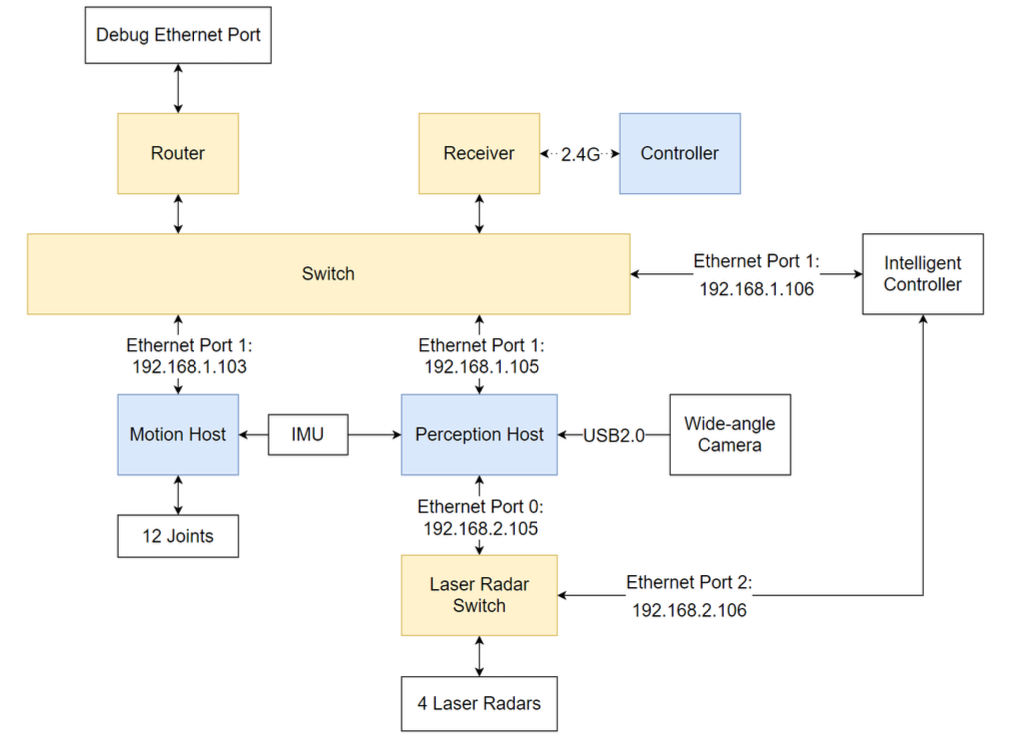
\includegraphics[width=0.65\textwidth]{gambar/bab2/network-x30.png}
  \caption{Arsitektur Jaringan Internal \emph{DeepRobotics Jueying X30 Pro} \cite{deeprobotics_jueyingx30}}
  \label{fig:network_architecture_x30pro}
\end{figure}

Gambar \ref{fig:network_architecture_x30pro} menunjukkan arsitektur modular dari Deep Robotics X30 Pro yang menggunakan jaringan Ethernet dan komunikasi nirkabel untuk menghubungkan berbagai komponen. Semua perangkat utama, termasuk \emph{Motion Host}, \emph{Perception Host}, \emph{IMU}, \emph{Laser Radar Switch}, dan \emph{Intelligent Controller}, saling terhubung melalui sebuah \emph{switch} yang berfungsi sebagai pusat distribusi data. \emph{Motion Host} berkomunikasi dengan 12 joints untuk mengendalikan gerakan robot, sedangkan \emph{Perception Host} mengelola input dari sensor, seperti kamera \emph{wide-angle} dan empat \emph{laser radars}. \emph{IMU} mengukur percepatan dan kecepatan sudut untuk memastikan navigasi yang stabil. Semua informasi ini diproses dan dikelola oleh \emph{Intelligent Controller} yang mengarahkan seluruh operasi robot. Robot ini memanfaatkan \emph{Robot Operating System (ROS) Noetic Ninjameys} yang dijalankan di sistem operasi \emph{Ubuntu 20.04}. \emph{ROS} memfasilitasi komunikasi antara berbagai perangkat keras dan perangkat lunak, memungkinkan integrasi yang mudah dengan sistem eksternal dan pengembangan aplikasi berbasis \emph{open-source}. Arsitektur jaringan yang terintegrasi ini mendukung efisiensi operasional dan memungkinkan pembaruan perangkat lunak yang lebih fleksibel, memperluas kemampuan dan potensi pengembangan robot.


\subsection{Hikvision HM-TD5528T-15/W}
Hikvision HM-TD5528T-15/W merupakan kamera pengawas tipe \emph{Thermographic Thermal and Optical Bi-spectrum Network Mini Positioning System} yang dirancang untuk pemantauan area kritis seperti gardu distribusi, fasilitas industri, dan zona rawan kebakaran. Kamera ini menggabungkan sensor termal dan sensor optik beresolusi tinggi dalam satu unit, serta didukung unit pemrosesan berbasis \emph{GPU} yang memungkinkan pemantauan suhu dan visual secara \emph{real-time}. Kamera ini menggunaka modul termal sensor \emph{Vanadium Oxide Uncooled Focal Plane Arrays} dengan resolusi \(256 \times 192\) piksel dan \emph{pixel pitch} \(12~\mu\text{m}\). Kamera ini memiliki sensitivitas termal tinggi dengan \emph{NETD} \(\leq 35~\text{mK}\) pada suhu \(25^\circ\text{C}\), dan dilengkapi lensa dengan panjang fokus 15~mm serta aperture F1.0. Sudut pandang termal sebesar \(11.69^\circ \times 8.78^\circ\) memberikan cakupan area yang cukup sempit namun presisi, dengan \emph{IFOV} \(0.8~\text{mrad}\) dan jarak fokus minimum 2{,}5~m. \emph{Zoom} digital tersedia hingga \(8 \times\).

Modul optik kamera ini menggunakan sensor \emph{CMOS} \(1/2.8^{\prime\prime}\) progresif dengan resolusi hingga 4~MP (\(2688 \times 1520\) piksel). Rentang panjang fokus optik adalah 4{,}8--153~mm, dengan \emph{optical zoom} hingga \(32 \times\) dan \emph{digital zoom} hingga \(16 \times\). Kamera ini juga mendukung fitur \emph{WDR} 120~dB, \emph{optical defog}, serta \emph{picture-in-picture} yang memungkinkan tampilan kanal termal ditampilkan bersamaan di kanal optik. Dalam hal pengukuran suhu, kamera ini menyediakan hingga 273 skenario yang masing-masing dapat memiliki hingga 21 aturan (10 titik, 10 area, dan 1 garis). Rentang suhu yang dapat diukur adalah dari \(-20^\circ\text{C}\) hingga \(550^\circ\text{C}\), dengan akurasi \(\pm 2^\circ\text{C}\) atau \(\pm 2\%\), tergantung nilai yang lebih besar. Kamera ini merupakan jenis kamera thermal \emph{CCTV} yang tidak memiliki konfigurasi nilai emisivitas secara langsung. Oleh karena itu, koreksi emisivitas perlu dilakukan secara eksternal, tergantung jenis permukaan target (contoh: logam teroksidasi sekitar 0{,}80, kulit manusia 0{,}95, keramik 0{,}90). Dari sisi integrasi sistem, perangkat ini mendukung berbagai protokol jaringan seperti \emph{IPv4/IPv6, RTSP, HTTP/HTTPS, ISAPI}, dan \emph{ONVIF (Profile S, G, T)}. Penyimpanan data dapat dilakukan melalui kartu \emph{microSD} hingga 128~GB dan \emph{NAS}, dengan dukungan fitur \emph{Automatic Network Replenishment (ANR)}. Kamera juga menyediakan antarmuka komunikasi seperti Ethernet \emph{RJ45} dan \emph{RS-485}, serta kompatibel dengan perangkat lunak pemantauan seperti iVMS-4200 dan Hik-Connect \cite{hikmicro_hmptz}.


\subsection{Doublecom DB6000FR-ANS}

Doublecom DB6000FR-ANS merupakan terminal nirkabel industri kelas luar ruang yang dirancang untuk lingkungan dengan mobilitas tinggi seperti kendaraan AGV, robot pintar, drone, dan sistem logistik otomatis. Perangkat ini mendukung standar komunikasi nirkabel IEEE 802.11a/n dan mengimplementasikan teknologi MIMO 2T2R dengan arsitektur dua antena pengirim dan penerima. DB6000FR-ANS memiliki bandwidth maksimum sebesar 300~Mbps dan daya pancar maksimum hingga 1000~mW. Perangkat ini juga dilengkapi dengan antarmuka \emph{RF} eksternal (2xSMA) yang memungkinkan penggunaan antena eksternal dengan berbagai karakteristik gain untuk meningkatkan jangkauan hingga lebih dari 1~km dalam kondisi tertentu. Sensitivitas penerimaannya mencapai \(-96~\text{dBm}\), yang menjadikannya cocok untuk komunikasi jarak jauh dan lingkungan padat interferensi.

Fitur utama lainnya mencakup dukungan \emph{Fast Roaming} (perpindahan AP dengan jeda kurang dari 50~ms), teknologi \emph{TDMA} untuk efisiensi dalam komunikasi multipoint, dan berbagai fungsi jaringan seperti \emph{VLAN, NAT, QoS, VPN}, serta \emph{firewall}. Selain itu, perangkat ini mendukung bandwidth fleksibel (5~MHz, 10~MHz, 20~MHz, dan 40~MHz), serta pengaturan spektrum dinamis melalui \emph{DFS}. Secara perangkat keras, DB6000FR-ANS dilengkapi prosesor 600~MHz, RAM 64~MB, dan antarmuka jaringan 10/100/1000BASE-T (RJ45). Desainnya tahan terhadap guncangan, antistatik, serta mampu bekerja dalam rentang suhu ekstrem antara \(-40^\circ\text{C}\) hingga \(75^\circ\text{C}\). Perangkat ini juga mendukung manajemen lokal maupun \emph{cloud} melalui platform aplikasi dan menyediakan indikator sinyal \emph{LED}, port \emph{PoE} 12--24~VDC, serta konsumsi daya maksimum hanya 9~W \cite{doublecom_db6000frans}.

\subsection{Doublecom DB6000ANLT90-FR}
Doublecom DB6000ANLT90-FR merupakan perangkat nirkabel luar ruang kelas operator (\emph{carrier-grade}) yang dirancang untuk menjadi titik pusat dalam komunikasi nirkabel berbasis sektor. Perangkat ini menggabungkan protokol IEEE 802.11a/n dengan antena \emph{dual-pol 90°} terintegrasi, bekerja dalam pita frekuensi 5.8~GHz bebas lisensi, mencakup rentang 5150--5850~MHz, dan memiliki gain antena sebesar 18~dBi. DB6000ANLT90-FR menggunakan arsitektur \emph{MIMO 2T2R} dengan kecepatan transmisi maksimum hingga 300~Mbps. Perangkat ini dirancang untuk komunikasi \emph{point-to-multipoint} dalam radius hingga 5~km, dan dapat mentransmisikan lebih dari 10 kanal video HD dengan bandwidth total lebih dari 100~Mbps. Ini dimungkinkan berkat penerapan teknologi \emph{TDMA} yang mengatur alokasi waktu transmisi antar titik secara efisien.

Dari sisi perangkat keras, perangkat ini dilengkapi \emph{CPU} 600~MHz, \emph{RAM} 64~MB, serta satu port jaringan RJ-45 berkecepatan 10/100/1000BASE-T. Power supply dapat disuplai melalui adaptor DC 12--24~V atau AC 200--300~V, serta mendukung \emph{PoE}. Fitur manajemen jaringan meliputi \emph{DHCP, VLAN, NAT, QoS, firewall, packet sniffing}, dan analisis lalu lintas secara langsung. Dari sisi ketahanan lingkungan, perangkat ini dilengkapi proteksi IP67 yang tahan air, angin, debu, dan paparan sinar matahari langsung. Perangkat dapat beroperasi dalam suhu \(-40^\circ\text{C}\) hingga \(75^\circ\text{C}\), kelembapan hingga 95\% (non-kondensasi), serta memiliki desain tahan guncangan dan disipasi panas. Konsumsi daya maksimum perangkat ini sekitar 14~W, dan dapat dipasang menggunakan bracket tipe-L atau sistem penjepit pipa berdiameter \(\phi 30{-}55~\text{mm}\) \cite{doublecom_db6000anlt90}.

\subsection{Moxa EDS-205}

Moxa EDS-205 adalah perangkat \emph{unmanaged Ethernet switch} industri dengan lima port RJ45 10/100BASE-T(X) yang mendukung mode \emph{auto negotiation} dan \emph{auto MDI/MDI-X}. Perangkat ini cocok untuk pengaplikasian di lingkungan industri karena mendukung standar IEEE 802.3, 802.3u, dan 802.3x, serta memiliki kemampuan proteksi terhadap \emph{broadcast storm} EDS-205 menggunakan metode pemrosesan \emph{store and forward}, memiliki ukuran tabel MAC sebesar 2K, dan \emph{buffer} paket sebesar 512~kbit. Perangkat ini beroperasi pada tegangan masukan 12--48~VDC, dengan konsumsi arus sekitar 0.12~A pada 24~VDC dan proteksi terhadap polaritas terbalik serta arus lebih (\(1.1~\text{A}\)). Dari sisi fisik, perangkat ini memiliki dimensi \(24.9 \times 100 \times 86.5~\text{mm}\), berat 135~g, dan dipasang melalui rel DIN. Perangkat ini dirancang dengan peringkat IP30 dan dapat beroperasi dalam suhu \(-10^\circ\text{C}\) hingga \(60^\circ\text{C}\), serta disertifikasi dengan berbagai standar keselamatan dan kompatibilitas elektromagnetik (seperti UL 508, EN 62368-1, EN 55032/35, IEC 61000-4-x). Perangkat ini sangat andal untuk kebutuhan komunikasi data industri yang tidak memerlukan konfigurasi kompleks \cite{moxa_eds205}.

\subsection{\emph{Robot Operating System (ROS)}}

\emph{Robot Operating System (ROS)} merupakan sebuah \emph{framework} perangkat lunak \emph{open-source} yang dikembangkan untuk memfasilitasi pengembangan aplikasi robotik yang modular dan skalabel. ROS menyediakan seperangkat \emph{tools} dan \emph{libraries} yang dirancang untuk mengelola berbagai fungsi utama dalam sistem robot, seperti kendali aktuator, pemrosesan data sensor, navigasi, dan perencanaan lintasan. Salah satu keunggulan utama ROS adalah arsitekturnya yang terdistribusi, memungkinkan pengembang untuk membagi sistem kompleks ke dalam unit-unit proses yang saling terhubung, dikenal sebagai \emph{node}. ROS mendukung beragam aplikasi, mulai dari robot industri hingga sistem otonom.Berikut merupakan komponen dan konsep fundamental yang membentuk arsitektur dan ekosistem ROS:

\subsubsection{2.2.7.1 \emph{Node}}
\emph{Node} adalah unit eksekusi dasar dalam ROS yang merepresentasikan sebuah proses independen untuk menjalankan tugas tertentu dalam sistem robot. Setiap \emph{node} memiliki tanggung jawab spesifik, seperti pembacaan data sensor atau pengendalian aktuator, dan dapat berkomunikasi dengan \emph{node} lainnya melalui mekanisme seperti \emph{topic}, \emph{service}, atau \emph{action}. Pendekatan ini memungkinkan sistem bekerja secara paralel dan modular.

\subsubsection{2.2.7.2 \emph{Topic}}
\emph{Topic} merupakan mekanisme komunikasi berbasis model \emph{publish/subscribe} yang memungkinkan pertukaran data antar \emph{node} secara asinkron. \emph{Node} yang berperan sebagai \emph{publisher} akan mengirimkan data ke suatu \emph{topic}, sedangkan \emph{subscriber} akan menerima data dari \emph{topic} tersebut. Data yang ditransmisikan berbentuk \emph{message} yang memiliki struktur dan tipe tertentu yang telah ditentukan.

\subsubsection{2.2.7.3 \emph{Service}}
\emph{Service} merupakan bentuk komunikasi sinkron antara dua \emph{node}, di mana satu \emph{node} mengirimkan permintaan (\emph{request}) dan \emph{node} lain memberikan tanggapan (\emph{response}) secara langsung. Mekanisme ini cocok untuk interaksi yang bersifat langsung dan satu kali, seperti pembacaan status atau perubahan konfigurasi.

\subsubsection{2.2.7.4 \emph{Action}}
\emph{Action} digunakan untuk menangani proses yang memerlukan waktu eksekusi yang relatif lama dan memungkinkan pemantauan progres secara kontinu. Berbeda dengan \emph{service} yang bersifat sinkron, \emph{action} menyediakan kemampuan komunikasi dua arah secara asinkron dengan dukungan umpan balik berkala (\emph{feedback}) serta notifikasi penyelesaian (\emph{result}).

\subsubsection{2.2.7.5 \emph{Launch File}}
\emph{Launch file} adalah berkas berformat XML yang digunakan untuk meluncurkan beberapa \emph{node} dan parameter konfigurasi secara bersamaan. File ini memungkinkan pengelolaan sistem ROS secara lebih efisien dan konsisten, terutama dalam pengujian dan pengoperasian sistem yang melibatkan banyak komponen secara paralel.

\subsubsection{2.2.7.6 \emph{Bag File}}
\emph{Bag file} merupakan format file dalam ROS yang digunakan untuk merekam dan memutar ulang data dari \emph{topic}. Fasilitas ini sangat berguna dalam pengujian, analisis, dan debugging karena memungkinkan simulasi ulang dari data historis tanpa perlu menjalankan robot secara langsung.

\subsubsection{2.2.7.7 \emph{Package}}
\emph{Package} adalah unit organisasi utama dalam ROS yang mengelompokkan \emph{node}, pustaka, dan file konfigurasi ke dalam satu kesatuan logis. Paket memfasilitasi pengembangan perangkat lunak yang terstruktur, modular, serta memudahkan distribusi dan pemeliharaan proyek dalam skala besar.

\subsubsection{2.2.7.8 \emph{Parameter}}
\emph{Parameter} adalah variabel konfigurasi yang disimpan dalam \emph{parameter server} ROS. Parameter ini memungkinkan \emph{node} untuk berbagi nilai konfigurasi secara global dalam sistem. Dengan memanfaatkan parameter, perubahan konfigurasi dapat dilakukan secara dinamis tanpa perlu memodifikasi kode sumber.

\subsubsection{2.2.7.9 \emph{Workspace}}
\emph{Workspace} adalah direktori kerja yang digunakan untuk mengelola pengembangan proyek ROS, termasuk penyimpanan kode sumber, hasil kompilasi, dan instalasi. Struktur \emph{workspace} umumnya mencakup folder \texttt{src}, \texttt{devel}, dan \texttt{install}, serta mendukung penggunaan \emph{catkin} sebagai sistem \emph{build} utama.

\subsubsection{2.2.7.10 \emph{Transformation (tf)}}
\emph{Transformation} adalah pustaka dalam ROS yang digunakan untuk melacak dan mengelola transformasi spasial antar kerangka koordinat (\emph{frame}) dalam sistem robot. Dengan \emph{tf}, pengembang dapat melakukan transformasi posisi dan orientasi antar objek atau sensor berdasarkan referensi waktu nyata. Pustaka ini menyediakan antarmuka seperti \texttt{tf::TransformListener} untuk mendengarkan transformasi dan \texttt{tf::TransformBroadcaster} untuk mempublikasikan transformasi antar \emph{frame}. Fitur ini sangat krusial dalam aplikasi navigasi, pemetaan, dan manipulasi objek, di mana presisi spasial menjadi aspek fundamental \cite{ros_noetic}.

\subsection{\emph{Localization dan Mapping}}

 \textit{ Localization and Mapping} berperan penting dalam sistem robotik dan kendaraan otonom, terutama dalam membangun peta lingkungan sekaligus menentukan posisi robot secara presisi. Seiring berkembangnya metode pemrosesan data LIDAR dan sensor IMU, berbagai pendekatan telah dikembangkan untuk meningkatkan akurasi, efisiensi komputasi, dan ketahanan terhadap dinamika lingkungan. 

\subsubsection{2.2.8.1 \emph{NanoGICP}}

\emph{NanoGICP} adalah algoritma \emph{registrasi cloud} point ringan yang dimodifikasi dari \emph{Generalized Iterative Closest Point (GICP)}. Algoritma ini menggabungkan pendekatan matriks \emph{kovarian} dalam \emph{GICP} dengan struktur data \emph{KD-tree} yang dioptimalkan untuk pemrosesan cepat. Dengan memanfaatkan estimasi kovarian yang teraproksimasi, \emph{NanoGICP} dapat menekan kompleksitas komputasi tanpa mengorbankan akurasi dan ketahanan terhadap data \emph{noise}. Hal ini menjadikannya sangat efisien dalam memproses data besar dengan waktu komputasi yang minim, sehingga ideal untuk aplikasi pada sistem dengan keterbatasan sumber daya komputasi. \emph{NanoGICP} sangat cocok diterapkan pada sistem \emph{LiDAR-based SLAM} yang dijalankan pada perangkat dengan keterbatasan komputasi, seperti robot berukuran kecil atau \emph{embedded systems}. Dengan kemampuannya yang ringan dan akurat, algoritma ini memungkinkan perangkat keras terbatas tetap dapat melakukan pemetaan dan lokalizasi secara efektif. \cite{koide2021nanogicp}.



\subsubsection{2.2.8.2 \emph{Quatro}}
\emph{Quatro} merupakan sistem lokalisasi berbasis \emph{LiDAR} yang mengintegrasikan empat strategi utama: \emph{scan-to-scan registration}, \emph{scan-to-map matching}, ekstraksi fitur bidang (\emph{plane-feature}), dan kompensasi deformasi waktu (\emph{time-deformed registration}). Kombinasi ini memungkinkan estimasi pose yang lebih akurat dan stabil dalam lingkungan yang dinamis serta berkontur kompleks. \emph{Quatro} terbukti memiliki performa unggul pada berbagai benchmark dataset seperti \emph{KITTI} dan \emph{NCLT}, serta mampu berjalan \emph{real-time} dengan efisiensi komputasi tinggi \cite{kim2022quatro}.


\subsubsection{2.2.8.3 \emph{Direct LiDAR-Inertial Odometry (DLIO)}}`
Algoritma \emph{Direct LiDAR-Inertia'l Odometry} (DLIO) menawarkan solusi dengan pendekatan \emph{coarse-to-fine} untuk menghasilkan koreksi gerakan waktu kontinu secara lebih akurat. DLIO memanfaatkan persamaan analitik yang dirancang untuk memperbaiki setiap titik data secara paralel dan efisien, sekaligus mengintegrasikan data LiDAR dan \emph{Inertial Measurement Unit} (IMU) secara ketat untuk menghasilkan estimasi keadaan robot yang lebih akurat. Pendekatan ini memungkinkan koreksi distorsi pada \emph{point cloud} secara \emph{real-time}, bahkan dalam kondisi pergerakan dinamis yang kompleks \cite{chen2022dlio}.


\begin{figure} [H] \centering
  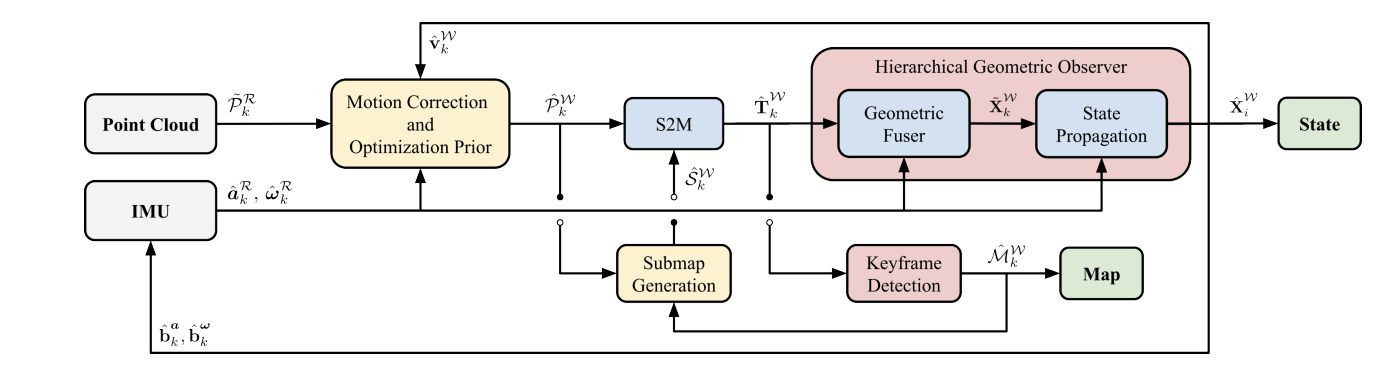
\includegraphics[scale=0.6]{gambar/bab2/dlio_Arch.png}
  \caption{Arsitektur \emph{Direct LiDAR-Inertial Odometry (DLIO)} \cite{chen2022dlio}}
  \label{fig:DLIO Architecture}
\end{figure}

Gambar \ref{fig:DLIO Architecture} menggambarkan arsitektur sistem \emph{Deep LiDAR Odometry and Mapping (DLIO)} yang menggabungkan berbagai komponen penting untuk estimasi posisi dan pembuatan peta. Sistem ini menerima input berupa \emph{point cloud} dari sensor LiDAR dan data dari \emph{IMU} (Inertial Measurement Unit), yang kemudian diproses untuk menghasilkan estimasi posisi dan peta 3D. Proses dimulai dengan koreksi gerakan dan pembuatan \emph{prior} berdasarkan data \emph{Point Cloud} dan \emph{IMU}. Selanjutnya, informasi ini dikirim ke \emph{S2M (Scan-to-Map)} untuk lebih mengoptimalkan peta yang dihasilkan. Hasilnya dikombinasikan dengan sistem \emph{Geometric Fuser} dalam \emph{Hierarchical Geometric Observer}, yang memfasilitasi penyempurnaan estimasi posisi melalui propagasi status. Peta yang dihasilkan kemudian diperbaharui dalam \emph{Submap Generation} dan \emph{Keyframe Detection}, yang membantu dalam pengolahan data lebih lanjut. Pada akhirnya, estimasi posisi dan peta 3D disajikan sebagai \emph{State} dan \emph{Map} yang terperinci.

Keunggulan DLIO tidak hanya terletak pada akurasi tinggi dalam estimasi posisi, tetapi juga pada efisiensi komputasi yang lebih baik dibandingkan dengan algoritma-algoritma terkini lainnya seperti \emph{LIO-SAM} dan \emph{FAST-LIO2}. DLIO menggabungkan koreksi gerakan dan pembuatan \emph{prior} dalam satu langkah, yang menghilangkan kebutuhan akan \emph{scan-to-scan matching} yang biasanya memakan waktu. Melalui eksperimen pada \emph{dataset} publik dan \emph{dataset} lapangan yang dikumpulkan secara mandiri, DLIO menunjukkan keunggulan dalam menghasilkan peta 3D yang detail dengan kesalahan posisi minimum. Sistem ini menjadi alternatif yang menjanjikan untuk platform robot bergerak, termasuk drone, dalam navigasi dan pemetaan di lingkungan yang tidak terstruktur.


Keunggulan DLIO tidak hanya terletak pada akurasi tinggi dalam estimasi posisi, tetapi juga pada efisiensi komputasi yang lebih baik dibandingkan algoritma-algoritma terkini lainnya seperti LIO-SAM dan FAST-LIO2. DLIO menggabungkan koreksi gerakan dan pembuatan \emph{prior} dalam satu langkah, menghilangkan kebutuhan akan \emph{scan-to-scan matching} yang biasanya memakan waktu. Melalui eksperimen pada \emph{dataset} publik dan \emph{dataset} lapangan yang dikumpulkan secara mandiri, DLIO menunjukkan keunggulan dalam menghasilkan peta 3D yang detail dengan kesalahan posisi minimum. Sistem ini menjadi alternatif yang menjanjikan untuk platform robot bergerak, termasuk drone, dalam navigasi dan pemetaan di lingkungan yang tidak terstruktur.



\subsubsection{2.2.8.4 \emph{Fast-LIO2}: \emph{Fast Direct LiDAR-Inertial Odometry}}

\emph{Fast-LIO2} adalah sistem \emph{LiDAR-Inertial Odometry} (\emph{LIO}) yang dirancang untuk efisiensi dan akurasi tinggi. Sistem ini menggunakan \emph{tightly-coupled iterated Kalman filter} dan dua inovasi utama: pertama, registrasi langsung titik-titik \emph{LiDAR} mentah ke peta voxel tanpa ekstraksi fitur eksplisit, sehingga menangkap detail lingkungan secara lebih halus dan fleksibel terhadap berbagai jenis \emph{LiDAR}; kedua, struktur data \emph{incremental k-d tree} (\emph{ikd-Tree}) yang mendukung pembaruan peta secara dinamis dan efisien, serta unggul dibanding \emph{octree}, \emph{R*-tree}, dan \emph{nanoflann}.

\begin{figure}[H]
    \centering
    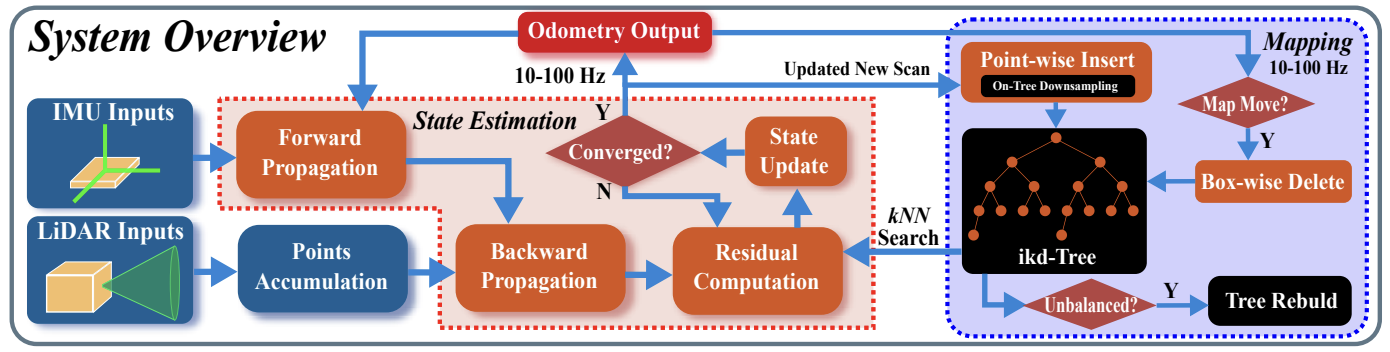
\includegraphics[width=1\textwidth]{gambar/bab2/fast-lio2.png}
    \caption{Diagram sistem \emph{Fast-LIO2}. \cite{xu2022fastlio}}
    \label{fig:fastlio2}
\end{figure}


Gambar \ref{fig:fastlio2} menunjukkan diagram sistem \emph{Fast-LIO2}, yang menggambarkan alur proses estimasi posisi dan pemetaan secara rinci. Sistem ini mengintegrasikan input dari \emph{IMU} (\emph{Inertial Measurement Unit}) dan \emph{LiDAR} untuk menghasilkan estimasi posisi yang akurat. Proses dimulai dengan akumulasi titik-titik \emph{LiDAR} yang diterima, yang kemudian diteruskan ke tahapan \emph{forward propagation} untuk melakukan estimasi status awal. Setelah itu, dilakukan \emph{backward propagation} yang diikuti dengan perhitungan residu untuk memperbarui status dengan lebih presisi. Kombinasi ini memungkinkan sistem untuk menghasilkan estimasi posisi yang sangat akurat dan peta lingkungan tiga dimensi yang sangat rinci. Selain itu, \emph{Fast-LIO2} menggunakan struktur data \emph{ikd-Tree} untuk memasukkan titik-titik secara langsung ke dalam peta dan melakukan pembaruan peta dengan cara yang efisien. Salah satu fitur unggulan dari \emph{ikd-Tree} adalah kemampuannya untuk melakukan \emph{on-tree downsampling}, yang mengurangi jumlah titik yang perlu diproses dan meningkatkan efisiensi komputasi secara keseluruhan. Dengan teknologi ini, \emph{Fast-LIO2} dapat berjalan dengan kecepatan tinggi dan menghasilkan peta yang sangat akurat. Sistem ini telah terbukti unggul dalam 19 sekuen \emph{dataset} publik dan mampu beroperasi hingga 100 Hz, bahkan dalam kondisi ekstrem seperti rotasi dengan kecepatan mencapai $1000^\circ/\text{s}$, yang membuatnya sangat cocok untuk aplikasi yang membutuhkan pemrosesan real-time dan akurasi tinggi, seperti navigasi robot dan kendaraan otonom \cite{xu2022fastlio}.




\subsubsection{2.2.8.5 \emph{Fast-LIO-SAM} sebagai Generator Peta}

\emph{Fast-LIO-SAM} adalah pengembangan dari \emph{Fast-LIO2} yang menggabungkan estimasi odometri berbasis \emph{LiDAR-Inertial Odometry} (\emph{LIO}) dengan backend optimisasi graf berbasis \emph{Smoothing and Mapping} (\emph{SAM}). Sistem ini memisahkan proses estimasi pose (\emph{frontend}) dan pemetaan serta koreksi \emph{loop closure (backend)}, sehingga mampu menghasilkan peta 3D yang konsisten dan akurat dalam skala besar. Salah satu keunggulan utama dari \emph{Fast-LIO-SAM} adalah kemampuannya untuk membangun dan menyimpan peta lingkungan dalam format data \texttt{.bag} (ROS bag file). Peta ini berisi informasi spasial hasil integrasi data \emph{LiDAR} dan \emph{IMU} yang telah dioptimasi secara global, dan dapat digunakan kembali untuk proses lokalisasi berulang di waktu yang berbeda tanpa perlu membangun ulang peta. Struktur peta voxel yang digunakan dalam \emph{backend SAM} membuat sistem ini efisien dalam konsumsi memori dan mendukung pemrosesan \emph{real-time}. Oleh karena itu, \emph{Fast-LIO-SAM} ideal digunakan sebagai tahap awal dalam pipeline sistem navigasi otonom, terutama ketika diperlukan peta dasar (\emph{prior map}) untuk aplikasi lokalisasi jangka panjang \cite{xu2022fastlio}.

\subsubsection{2.2.8.6 \emph{Fast-LIO Localization QN}: Integrasi \emph{Quatro} dan \emph{NanoGICP}}

\emph{Fast-LIO Localization QN} adalah sistem lokalisasi berbasis peta yang dirancang untuk bekerja dengan peta hasil dari sistem seperti \emph{Fast-LIO-SAM}. Peta yang telah dibangun dan disimpan dalam format \texttt{.bag} melalui proses SLAM sebelumnya akan digunakan sebagai referensi untuk melakukan lokalisasi kembali terhadap data \emph{LiDAR} baru. Pendekatan ini memungkinkan navigasi yang presisi dan efisien tanpa harus melakukan pemetaan ulang secara terus-menerus.Arsitektur QN menggabungkan modul odometri dari \emph{Fast-LIO2} dengan dua komponen utama dalam proses \emph{map matching}, yaitu \emph{Quatro} dan \emph{NanoGICP}. \emph{Quatro} digunakan untuk melakukan registrasi global cepat, yang memberikan perkiraan awal transformasi posisi sensor terhadap peta. Hal ini sangat penting dalam skenario dengan deviasi posisi awal besar atau ketika sistem baru aktif. Setelah diperoleh transformasi awal, \emph{NanoGICP} digunakan untuk proses refinemen lokal. Algoritma ini merupakan kombinasi dari \emph{FastGICP} dan \emph{NanoFLANN}, yang memungkinkan pencocokan lokal secara presisi tinggi dengan beban komputasi rendah. Integrasi ini memungkinkan proses lokalisasi yang cepat, akurat, dan tahan terhadap noise lingkungan. Karena \emph{QN} tidak melakukan pemetaan ulang, sistem ini sangat cocok untuk digunakan dalam skenario di mana peta telah tersedia, seperti area industri, fasilitas logistik, gudang, dan bangunan besar dengan struktur tetap. Sistem ini juga mempercepat waktu inisialisasi dan mengurangi konsumsi sumber daya komputasi, karena hanya fokus pada lokalisasi berbasis peta referensi yang diberikan\cite{fastlio2023qnloc}.


\subsection{\emph{Navigation}}
\emph{Path navigation} merupakan komponen kunci dalam sistem robotik bergerak otonom. Komponen ini bertugas memastikan bahwa robot dapat mengikuti jalur yang telah direncanakan sekaligus mampu bereaksi terhadap dinamika lingkungan seperti rintangan statis maupun bergerak. Pendekatan navigasi umumnya dibagi menjadi dua: pengendalian jalur (\emph{path following}) dan penghindaran rintangan (\emph{obstacle avoidance}). Dalam subbagian ini dibahas tiga pendekatan utama yang sering digunakan dan relevan untuk integrasi sistem navigasi cerdas, yaitu \emph{PID controller}, \emph{Braitenberg-based obstacle avoidance}, dan \emph{Pure Pursuit}.

\subsubsection{2.2.9.1 \emph{PID Controller}}

Pengendali PID (\emph{Proportional-Integral-Derivative}) merupakan salah satu algoritma kontrol klasik yang masih luas digunakan karena kesederhanaannya dan efektivitasnya dalam berbagai aplikasi sistem dinamis. PID terdiri dari tiga komponen utama yang bekerja secara sinergis dalam mengurangi kesalahan (\emph{error}) antara nilai keluaran aktual dan nilai referensi sistem. Komponen  \emph{proportional} (\(P\)), memberikan respons sebanding terhadap besarnya \emph{error} saat ini. Semakin besar \emph{error}, semakin besar koreksi yang diberikan, yang membantu sistem mendekati set point secara langsung. Komponen  \emph{integral} (\(I\)), menjumlahkan \emph{error} dari waktu ke waktu untuk mengoreksi kesalahan tetap (\emph{steady-state error}) yang tidak bisa dihilangkan hanya dengan kontrol \emph{proportional}. Komponen \emph{derivative} (\(D\)), bertindak berdasarkan laju perubahan \emph{error}, memberikan peredaman (\emph{damping}) terhadap respons sistem, dan mengurangi gejala \emph{overshoot} serta mempercepat  (\emph{rise time}) menuju \emph{set point}. Secara matematis, sinyal kontrol total \( u(t) \) dalam pengendali PID dapat dirumuskan sebagai:
\begin{equation}
    u(t) = K_p e(t) + K_i \int_{0}^{t} e(\tau) \, d\tau + K_d \frac{d}{dt}e(t),
\end{equation}
di mana \( K_p \), \( K_i \), dan \( K_d \) masing-masing adalah konstanta penguatan (\emph{gain}) untuk komponen \emph{proportional}, \emph{integral}, dan \emph{derivative}, dan \( e(t) \) adalah sinyal kesalahan pada waktu \( t \). Dalam konteks navigasi jalur, pengendali PID umum digunakan untuk mengatur kecepatan linier dan sudut belok robot berdasarkan \emph{cross-track error} (deviasi lateral terhadap jalur) dan \emph{heading error} (perbedaan orientasi). Parameter PID yang dituning dengan baik dapat meminimalkan \emph{steady-state error}, mengontrol \emph{overshoot}, serta mempercepat \emph{rise time} menuju kondisi stabil. Namun, dalam lingkungan yang sangat dinamis atau nonlinear, efektivitas PID dapat menurun karena sifatnya yang tidak adaptif terhadap perubahan konteks \cite{astrom1995pid}.


\subsubsection{2.2.9.2 \emph{Braitenberg Obstacle Avoidance}}

Penghindaran rintangan berdasarkan prinsip \emph{Braitenberg} merupakan pendekatan reaktif yang meniru perilaku biologis sederhana. Dalam pendekatan ini, sensor, seperti sensor ultrasonik atau \emph{LiDAR}, dihubungkan langsung ke aktuator secara fungsional, yang memungkinkan robot untuk bereaksi terhadap objek yang terdeteksi di sekitarnya. Dalam bentuk dasar, intensitas pembacaan sensor mempengaruhi kecepatan roda secara langsung, dengan tujuan menghindari objek yang terdeteksi tanpa memerlukan perhitungan kompleks atau pembuatan peta. Sebagai contoh, jika sensor mendeteksi objek di depan, robot akan memperlambat roda yang berada di sisi yang lebih dekat dengan objek, memutar arah untuk menghindari tabrakan. Meskipun pendekatan ini sangat sederhana, ia terbukti sangat efektif dalam situasi yang memerlukan penghindaran rintangan di lingkungan yang tidak terstruktur. Pendekatan \emph{Braitenberg} sering digunakan pada robot yang bergerak dalam area yang dinamis, di mana reaksi cepat terhadap perubahan lingkungan sangat penting. Namun, karena sifatnya yang reaktif, metode ini cenderung menghasilkan gerakan yang tidak halus dan terkadang tidak optimal, terutama dalam navigasi jalur yang kompleks. Robot yang menggunakan pendekatan ini mungkin akan kesulitan saat menghadapi jalur yang harus dilalui dengan presisi tinggi atau di lingkungan yang memiliki banyak hambatan. Oleh karena itu, \emph{Braitenberg} sering digunakan sebagai lapisan reaktif tambahan pada sistem pengendalian berbasis jalur, seperti \emph{PID} atau \emph{Pure Pursuit}, untuk meningkatkan respons terhadap rintangan secara real-time sambil mempertahankan kontrol navigasi yang lebih halus dan terencana. Kombinasi ini memungkinkan robot untuk memiliki respons cepat terhadap rintangan, sambil tetap mengikuti jalur. \cite{braitenberg1986vehicles}.


\subsubsection{2.2.9.3 Pure Pursuit untuk Pelacakan Jalur}

\emph{Pure Pursuit} adalah algoritma pelacakan jalur berbasis geometri yang dirancang untuk mengarahkan robot menuju sebuah titik target (\emph{look-ahead point}) yang berada di depan lintasan referensi. Algoritma ini populer karena kesederhanaannya serta kemampuannya menghasilkan lintasan yang halus, terutama pada sistem robotik non-ackermann seperti robot dengan \emph{differential drive}. Prinsip kerja \emph{Pure Pursuit} adalah membentuk lintasan lengkung dari posisi robot menuju titik target. Sudut belok atau kelengkungan lintasan dihitung berdasarkan sudut \( \alpha \), yaitu sudut antara arah heading robot saat ini dan garis lurus ke titik target, serta jarak \emph{look-ahead} \(L_d\). Kelengkungan lintasan ditentukan oleh persamaan:
\begin{equation}
    \kappa = \frac{2 \cdot \sin(\alpha)}{L_d},
\end{equation}
di mana \( \kappa \) kemudian dikonversi menjadi kecepatan sudut:
\begin{equation}
    \omega = v \cdot \kappa,
\end{equation}
dengan \( v \) adalah kecepatan linier robot.

\emph{Look ahed distance} \(L_d\) sangat memengaruhi karakteristik gerakan yang dihasilkan oleh algoritma ini. Ketika nilai \(L_d\) terlalu kecil, robot menjadi sangat responsif terhadap perubahan arah, sehingga sering kali menghasilkan lintasan yang terlalu tajam atau osilatif, terutama pada kecepatan tinggi. Sebaliknya, jika \(L_d\) terlalu besar, robot cenderung mengambil jalur yang lebih lurus dan memotong tikungan, sehingga berpotensi menyimpang dari lintasan referensi. Oleh karena itu, pemilihan nilai \(L_d\) perlu mempertimbangkan kecepatan dan konteks lingkungan. Beberapa implementasi bahkan menggunakan skema adaptif yang menyesuaikan \(L_d\) secara dinamis seiring dengan kecepatan robot untuk menjaga keseimbangan antara stabilitas dan akurasi pelacakan. Metode \emph{Pure Pursuit} sangat cocok untuk navigasi jalur dengan geometri kompleks karena mampu menyesuaikan arah gerak secara kontinu berdasarkan posisi dan heading saat ini. Untuk meningkatkan stabilitas sistem dan mengurangi osilasi gerakan, algoritma ini sering dikombinasikan dengan pengendali PID yang mengatur kecepatan sudut berdasarkan nilai kelengkungan yang dihitung \cite{coulter1992implementation}.


\subsection{\emph{Computer Vision}}

\emph{Computer vision} merupakan cabang dari kecerdasan buatan yang bertujuan untuk memungkinkan komputer memahami dan menganalisis informasi dari citra maupun video digital. Tidak seperti manusia yang secara intuitif dapat mengenali objek, memperkirakan jarak, dan memahami konteks visual, sistem \emph{computer vision} memerlukan algoritma matematis dan pemrograman tingkat lanjut untuk meniru proses tersebut. Salah satu perkembangan penting dalam bidang ini adalah penggunaan arsitektur \emph{Convolutional Neural Network} (CNN), yang menjadi fondasi dalam berbagai aplikasi seperti klasifikasi citra, segmentasi semantik, serta deteksi objek. Salah satu algoritma deteksi objek yang paling populer adalah \emph{You Only Look Once} (YOLO). YOLO telah mengalami banyak peningkatan sejak pertama kali diperkenalkan pada tahun 2016, dengan tujuan untuk meningkatkan kecepatan dan akurasi deteksi objek dalam citra. YOLO bekerja dengan membagi citra menjadi grid dan memprediksi bounding box serta kelas objek dalam satu langkah pemrosesan, menjadikannya sangat efisien untuk aplikasi \emph{real-time}.


\subsubsection{2.2.10.1 YOLOv8}
\emph{YOLOv8} merupakan pengembangan dari algoritma \emph{You Only Look Once} yang menggunakan pendekatan deteksi satu tahap (\emph{one-stage detection}). Model ini mendeteksi objek secara langsung dari keseluruhan citra dalam satu proses, tanpa perlu memisahkannya menjadi beberapa bagian seperti pada metode dua tahap. Peningkatan utama pada \emph{YOLOv8} meliputi optimasi deteksi multi-skala, penggunaan \emph{backbone} yang efisien seperti \emph{CSPDarknet}, serta \emph{neck} yang ditingkatkan untuk ekstraksi fitur, seperti \emph{PANet}. Arsitektur ini memungkinkan deteksi yang cepat dan akurat, serta efisien untuk diterapkan pada perangkat dengan daya komputasi terbatas.  Dengan kombinasi kecepatan, akurasi, dan efisiensi, \emph{YOLOv8} banyak digunakan dalam berbagai aplikasi \emph{computer vision}, termasuk sistem keamanan, kendaraan otonom, dan pengolahan citra medis \cite{yolov8}.


\subsubsection{2.2.10.2 \emph{OpenVINO}}
\emph{OpenVINO (Open Visual Inference and Neural Network Optimization)} adalah toolkit dari Intel yang dirancang untuk mempercepat inferensi model \emph{deep learning} pada perangkat keras yang berbeda, termasuk \emph{CPU, GPU}, dan \emph{VPU}. Dengan menggunakan \emph{OpenVINO}, model \emph{YOLOv8} dapat dioptimalkan untuk berjalan pada perangkat \emph{edge} dengan efisiensi tinggi. \emph{OpenVINO} mendukung berbagai format model, termasuk \emph{TensorFlow, PyTorch}, dan \emph{ONNX}, serta menyediakan alat untuk konversi model ke format \emph{Intermediate Representation (IR)} yang lebih efisien. Selain itu, \emph{OpenVINO} juga menawarkan optimasi presisi data seperti \emph {\texttt{FP16} (16-bit floating point)} dan \emph{\texttt{INT8} (8-bit integer)}, yang memungkinkan peningkatan performa inferensi dengan kompromi minimal terhadap akurasi. Dengan demikian, \emph{OpenVINO} sangat cocok untuk aplikasi \emph{real-time} seperti pemantauan suhu termal pada gardu listrik \cite{openvino2021toolkit}.

\subsection{Metode Evaluasi dalam \emph{Computer Vision}}

Evaluasi performa model dalam \emph{computer vision} sangat penting untuk mengukur efektivitas sistem dalam mendeteksi dan mengklasifikasikan objek secara akurat. Beberapa metrik evaluasi yang umum digunakan meliputi \emph{confusion matrix}, \emph{precision}, \emph{recall}, \emph{accuracy}, \emph{F1 score}, dan \emph{loss function}. Masing-masing metrik memberikan perspektif yang berbeda mengenai kinerja model, baik dari segi akurasi keseluruhan, kesalahan klasifikasi, maupun keseimbangan antara kesalahan positif dan negatif.

\subsubsection{2.2.11.1 \emph{Confusion Matrix}}

\emph{Confusion matrix} adalah alat yang sangat berguna dalam evaluasi kinerja model klasifikasi, terutama dalam konteks pembelajaran mesin dan statistik. Matriks ini memberikan gambaran yang jelas tentang kinerja model dalam hal prediksi benar dan salah untuk setiap kelas. Umumnya, \emph{confusion matrix} digunakan untuk mengevaluasi model klasifikasi biner, namun dapat juga diperluas untuk masalah klasifikasi multikelas dengan menambah jumlah baris dan kolom sesuai dengan jumlah kelas.

Pada klasifikasi biner, \emph{confusion matrix} terdiri dari empat komponen utama yang menggambarkan hasil prediksi model. Pertama, \emph{True Positive (TP)} menunjukkan jumlah data yang benar-benar positif dan diprediksi sebagai positif oleh model. Sebagai contoh, dalam sistem deteksi penyakit, \emph{TP} mengacu pada jumlah pasien yang benar-benar sakit dan diprediksi sebagai sakit oleh model. Kedua, \emph{True Negative (TN)} adalah jumlah data yang benar-benar negatif dan diprediksi sebagai negatif. Dalam contoh yang sama, \emph{TN} merujuk pada jumlah pasien yang sehat dan diprediksi sehat oleh model.

Ketiga, \emph{False Positive (FP)} merujuk pada jumlah data negatif yang salah diprediksi sebagai positif. Dalam deteksi penyakit, ini adalah jumlah pasien yang sebenarnya sehat tetapi diprediksi sakit oleh model, yang dikenal sebagai \emph{false alarm}. Keempat, \emph{False Negative (FN)} merujuk pada jumlah data positif yang salah diprediksi sebagai negatif. Dalam hal ini, \emph{FN} adalah jumlah pasien yang sakit tetapi diprediksi sehat oleh model, yang dapat menyebabkan masalah serius karena pengabaian penyakit.

\begin{figure}[H]
  \centering
  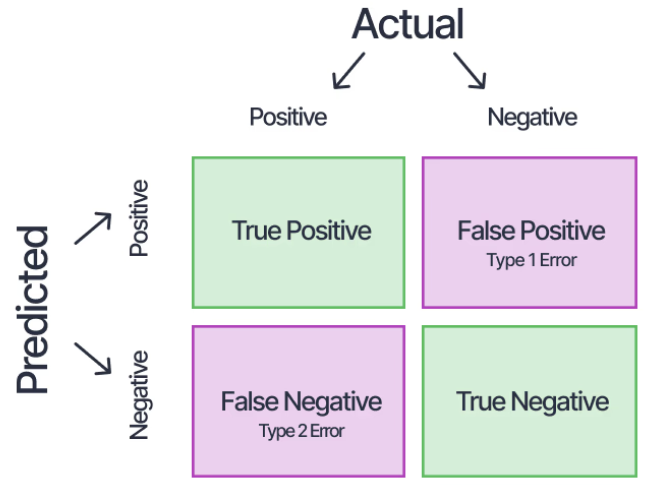
\includegraphics[scale=0.7]{gambar/bab2/cf.png}
  \caption{Contoh \emph{confusion matrix} untuk klasifikasi biner.\cite{V7Labs2025}}
  \label{fig:cf}
\end{figure}

Gambar \ref{fig:cf} menunjukkan contoh dari \emph{confusion matrix} untuk klasifikasi biner, yang memperlihatkan bagaimana komponen-komponen tersebut dihitung dan digunakan untuk mengevaluasi kinerja model. Melalui analisis ini, kita bisa menghitung berbagai metrik evaluasi lainnya, seperti \emph{accuracy}, \emph{precision}, \emph{recall}, dan \emph{F1-score}, yang memberikan gambaran lebih menyeluruh tentang performa model dalam memprediksi kelas. Melalui analisis terhadap keempat komponen ini, pengguna dapat mengevaluasi secara lebih mendalam jenis kesalahan yang terjadi pada model, seperti kecenderungan overfitting terhadap kelas tertentu atau ketidakseimbangan prediksi. Informasi dari \emph{confusion matrix} juga menjadi dasar dalam perhitungan metrik evaluasi lain seperti \emph{accuracy}, \emph{precision}, \emph{recall}, dan \emph{F1-score}, yang lebih menggambarkan performa model secara menyeluruh dalam konteks prediksi klasifikasi \cite{V7Labs2025}.

\subsubsection{A. \emph{Precision}, \emph{Recall}, dan \emph{Accuracy}}

\emph{Precision} adalah metrik yang digunakan untuk mengukur seberapa akurat prediksi positif yang dilakukan oleh model. Metrik ini penting ketika kita ingin meminimalkan kesalahan \emph{false positive}, yaitu prediksi yang salah mengklasifikasikan data negatif sebagai positif. Rumus untuk menghitung \emph{precision} adalah sebagai berikut:

\begin{equation}
  \text{Precision} = \frac{TP}{TP + FP}
\end{equation}

Di mana \( TP \) (\emph{True Positive}) adalah jumlah data positif yang benar-benar diprediksi positif oleh model, dan \( FP \) (\emph{False Positive}) adalah jumlah data negatif yang salah diprediksi sebagai positif oleh model. Metrik ini mengukur proporsi prediksi positif yang benar-benar akurat. \emph{Recall}, di sisi lain, mengukur seberapa banyak data positif yang berhasil dikenali oleh model. Metrik ini penting untuk meminimalkan kesalahan \emph{false negative}, yaitu ketika data positif diprediksi sebagai negatif. Rumus untuk \emph{recall} adalah:

\begin{equation}
  \text{Recall} = \frac{TP}{TP + FN}
\end{equation}

Di mana \( FN \) (\emph{False Negative}) adalah jumlah data positif yang salah diprediksi sebagai negatif oleh model. \emph{Recall} mengukur sejauh mana model dapat mendeteksi seluruh data positif yang sebenarnya ada dalam dataset. Sedangkan \emph{Accuracy} adalah metrik yang mengukur persentase keseluruhan prediksi yang benar, baik positif maupun negatif. \emph{Accuracy} memberikan gambaran umum tentang seberapa baik model dalam melakukan prediksi secara keseluruhan. Rumus untuk menghitung \emph{accuracy} adalah:

\begin{equation}
  \text{Accuracy} = \frac{TP + TN}{TP + TN + FP + FN}
\end{equation}

\emph{ TN  (True Negative)} adalah jumlah data negatif yang diprediksi sebagai negatif oleh model. Metrik ini memberikan ukuran tingkat kesalahan secara keseluruhan, tetapi tidak selalu mencerminkan kinerja model dengan baik, terutama jika ada ketidakseimbangan kelas\cite{V7Labs2025}.

\subsubsection{B. \emph{F1 Score}}

\emph{F1 score} adalah metrik yang memberikan gambaran lebih baik tentang keseimbangan antara \emph{precision} dan \emph{recall}, terutama ketika ada ketidakseimbangan kelas dalam dataset. \emph{F1 score} adalah rata-rata harmonis antara \emph{precision} dan \emph{recall}, yang berarti bahwa metrik ini akan memberikan nilai rendah jika salah satu dari keduanya rendah. \emph{F1 score} digunakan ketika kita ingin menyeimbangkan kedua metrik ini, agar model tidak hanya fokus pada satu metrik saja. Rumus untuk menghitung \emph{F1 score} adalah sebagai berikut:

\begin{equation}
  F_1 = 2 \times \frac{\text{Precision} \times \text{Recall}}{\text{Precision} + \text{Recall}}
\end{equation}

 \emph{F1 score} memberikan nilai yang lebih baik ketika \emph{precision} dan \emph{recall} memiliki nilai yang seimbang, dan lebih sensitif terhadap nilai rendah di salah satu metrik. Ini sangat berguna ketika data memiliki distribusi kelas yang tidak seimbang, di mana salah satu kelas lebih dominan daripada yang lainnya \cite{V7Labs2025}.

\subsubsection{C. \emph{Loss Function}}

\emph{Loss function} adalah fungsi yang digunakan untuk mengukur seberapa jauh prediksi model dari nilai sebenarnya (\emph{ground truth}). Dalam konteks pelatihan model pembelajaran mesin, \emph{loss function} digunakan untuk menghitung kesalahan prediksi, dan tujuan utama dalam pelatihan adalah untuk meminimalkan nilai loss ini agar model dapat melakukan prediksi yang lebih baik. Salah satu fungsi kerugian yang paling umum digunakan dalam klasifikasi adalah \emph{cross-entropy loss} \cite{V7Labs2025}.

\begin{equation}
L = -\sum_{i=1}^{C} y_i \log(p_i)
\end{equation}

\emph{C} adalah jumlah kelas dalam masalah klasifikasi, \( y_i \) adalah label asli untuk kelas ke-\(i\) yang bernilai 1 jika data tersebut termasuk dalam kelas tersebut dan 0 jika tidak. \( p_i \) adalah probabilitas prediksi model terhadap kelas ke-\(i\), yang dihitung oleh model menggunakan fungsi aktivasi seperti \emph{softmax} pada output.   Fungsi \emph{cross-entropy loss} ini mengukur jarak antara distribusi probabilitas yang diprediksi oleh model dan distribusi probabilitas yang sebenarnya (\emph{ground truth}). Nilai \emph{loss} yang lebih kecil menunjukkan bahwa model lebih baik dalam memprediksi kelas yang benar, sedangkan nilai \emph{loss} yang lebih besar menunjukkan bahwa prediksi model jauh dari nilai yang sebenarnya. Fungsi ini sangat penting dalam klasifikasi karena mengoptimalkan prediksi probabilitas dan meminimalkan kesalahan klasifikasi. \emph{Cross-entropy loss} sangat berguna dalam pelatihan jaringan saraf, karena dapat menangani klasifikasi multikelas dan memberikan gambaran yang lebih akurat tentang seberapa baik model dalam memprediksi kelas yang benar dengan mempertimbangkan ketidakpastian dalam prediksi tersebut.



\subsection{\emph{Web GUI}}

\emph{Web Graphical User Interface} atau \emph{Web GUI} merupakan evolusi dari antarmuka pengguna tradisional yang umumnya dijalankan melalui aplikasi desktop. Dengan memanfaatkan teknologi web, \emph{Web GUI} memungkinkan pengguna untuk berinteraksi dengan sistem atau aplikasi melalui peramban \emph{website} (\emph{browser}) tanpa memerlukan instalasi perangkat lunak tambahan, sehingga memberikan fleksibilitas tinggi dan aksesibilitas yang luas \cite{krug2014dont}. Keunggulan utama dari \emph{Web GUI} dibandingkan dengan \emph{GUI} konvensional terletak pada sifatnya yang lintas platform dan berbasis cloud. Selama pengguna memiliki koneksi internet dan peramban modern, aplikasi dapat diakses secara langsung tanpa bergantung pada sistem operasi tertentu \cite{murugesan2007web}. Selain itu, proses pemeliharaan dan pembaruan (\emph{update}) menjadi lebih efisien, karena seluruh perubahan dapat dilakukan secara terpusat pada sisi server tanpa perlu mendistribusikan ulang perangkat lunak kepada setiap pengguna. Dalam konteks pengembangan sistem modern, \emph{Web GUI} sangat didukung oleh berbagai teknologi berbasis \emph{JavaScript} dan framework pendukung yang memungkinkan pengembangan antarmuka yang cepat, responsif, dan \emph{scalable}. 

\subsubsection{2.2.12.1 React.js}

React.js merupakan salah satu \emph{library} \emph{JavaScript} yang umum digunakan dalam pengembangan antarmuka pengguna (\emph{user interface}) yang dinamis dan interaktif. React mengadopsi pendekatan berbasis \emph{component}, yaitu unit antarmuka yang terpisah dan modular, sehingga memudahkan proses pengembangan, pemeliharaan, serta pengujian perangkat lunak. Komponen dalam React dapat dibangun melalui dua pendekatan utama, yaitu \emph{class components} dan \emph{functional components}, yang keduanya bertanggung jawab dalam proses \emph{rendering} elemen antarmuka berdasarkan \emph{props} dan \emph{state} \cite{Panjaitan2021}. Efisiensi dalam pembaruan antarmuka didukung oleh penerapan \emph{Virtual DOM}, yang memungkinkan perubahan hanya terjadi pada bagian yang terdampak tanpa memuat ulang seluruh halaman. Pendekatan ini tidak hanya meningkatkan keterbacaan dan perawatan kode, tetapi juga mendukung prinsip \emph{reusability}, yakni penggunaan kembali komponen di berbagai konteks pengembangan. Dengan karakteristik tersebut, React.js menjadi salah satu teknologi dominan dalam pengembangan aplikasi web berbasis \emph{single-page application} (\emph{SPA}) \cite{Panjaitan2021}.

\subsubsection{2.2.12.2 Next.js}
Next.js merupakan \emph{framework} berbasis \emph{React} yang dikembangkan untuk mendukung pengembangan aplikasi web \emph{full-stack} secara efisien dan terstruktur. Sebagai ekstensi dari \emph{React}, Next.js menyederhanakan berbagai konfigurasi tingkat rendah seperti \emph{module bundling}, \emph{routing}, dan \emph{code splitting}, yang umumnya memerlukan pengaturan manual dalam proyek \emph{React} murni \cite{Nextjs2024}. Kemampuan ini memungkinkan pengembang untuk fokus pada pengembangan fitur tanpa harus terlibat langsung dalam proses pengelolaan infrastruktur aplikasi. Next.js mengintegrasikan secara native pendekatan \emph{server-side rendering (SSR)} dan \emph{static site generation (SSG)}, dua teknik rendering yang krusial dalam optimalisasi performa dan aksesibilitas halaman web. \emph{SSR} memungkinkan halaman dirender di sisi server sebelum dikirim ke klien, sehingga mengurangi waktu muat awal pada web browswer. Di sisi lain, \emph{SSG} menghasilkan halaman statis pada waktu kompilasi, yang secara signifikan menurunkan beban server dan mempercepat distribusi konten. Kombinasi kedua pendekatan ini memberikan fleksibilitas tinggi dalam strategi rendering berdasarkan kebutuhan spesifik aplikasi. Dalam konteks pengembangan berbasis komponen, integrasi React dan Next.js mendukung pengembangan antarmuka interaktif dengan performa tinggi. Studi mutakhir menunjukkan bahwa implementasi \emph{framework} seperti Next.js dapat menurunkan latensi interaksi, meningkatkan \emph{user engagement}, serta mendukung skalabilitas dalam arsitektur perangkat lunak modern \cite{Nextjs2024}.

\subsubsection{2.2.12.3 Tailwind CSS}

Tailwind CSS merupakan \emph{framework} \emph{utility-first} berbasis CSS yang mengedepankan penggunaan kelas utilitas langsung dalam markup untuk membentuk antarmuka pengguna yang responsif dan terstruktur. Berbeda dengan \emph{framework} tradisional yang menyediakan komponen siap pakai, pendekatan Tailwind memungkinkan fleksibilitas tinggi dan iterasi cepat dalam pengembangan desain kustom \cite{Azhariyah2024}. Integrasinya yang seamless dengan \emph{framework JavaScript} seperti React dan Angular memperkuat efisiensi pengembangan berbasis komponen, sekaligus mengurangi kebutuhan akan file \emph{CSS} yang besar. Dukungan bawaan terhadap desain responsif menjadikan Tailwind CSS relevan untuk pengembangan aplikasi lintas perangkat dengan konsistensi visual yang tinggi.

\subsubsection{2.2.12.4 ShadCN}

ShadCN UI merupakan kumpulan komponen \emph{React} modern yang bersifat \emph{open-source}, namun tidak dikemas sebagai pustaka tradisional yang dapat diinstal melalui \emph{Node Package Manager} (\emph{npm}). Sebaliknya, pengembang menyalin langsung kode sumber komponen ke dalam basis kode proyek, sehingga memberikan fleksibilitas tinggi dalam modifikasi fungsionalitas dan penataan. Komponen-komponen ini menggunakan \emph{Tailwind CSS} untuk styling, dengan desain awal yang konsisten dan minimalis. ShadCN menyediakan beragam komponen antarmuka umum seperti \emph{dialog}, \emph{input}, \emph{checkbox}, dan \emph{table}, serta mendukung integrasi cepat melalui perintah \emph{CLI} untuk menyalin kode ke dalam direktori lokal proyek \cite{Shadcn2024}. Pendekatan ini menghasilkan aplikasi yang lebih ringan dan modular, karena hanya menyertakan komponen yang benar-benar dibutuhkan.

\subsubsection{2.2.12.4 Express.js}
Express.js adalah \emph{framework} minimalis untuk Node.js yang dirancang untuk membangun aplikasi web dan API dengan cepat dan efisien. Dengan arsitektur yang sederhana dan fleksibel, Express memungkinkan pengembang untuk membuat aplikasi dengan struktur yang jelas dan mudah dipelihara. Salah satu fitur utama dari Express adalah kemampuannya untuk menangani berbagai jenis permintaan \emph{HTTP}, serta mendukung \emph{middleware} yang memungkinkan penanganan permintaan secara modular. Middleware ini dapat digunakan untuk berbagai tujuan, seperti otentikasi, pengolahan data, dan penanganan kesalahan \cite{express2023docs}. Selain itu, Express juga memiliki ekosistem yang luas dengan banyak pustaka tambahan yang dapat diintegrasikan untuk memperluas fungsionalitas aplikasi. Dengan demikian, Express.js menjadi pilihan populer bagi pengembang yang ingin membangun aplikasi web modern dengan cepat dan efisien.

\subsubsection{2.2.12.5 PostgreSQL}
PostgreSQL, sebuah sistem manajemen basis data relasional 
\emph{(RDBMS)} \emph{open-source} yang terkenal, telah menjadi pilihan utama dalam pengembangan aplikasi berbasis data. Dengan arsitektur dan  dukungan untuk berbagai fitur, PostgreSQL menawarkan kemampuan yang sangat baik dalam hal penyimpanan, pengambilan, dan manipulasi data. Sistem ini dikenal karena kepatuhannya terhadap standar SQL, serta kemampuannya untuk menangani transaksi kompleks dengan tingkat konsistensi yang tinggi \cite{postgresql2023docs}. PostgreSQL juga mendukung berbagai tipe data, termasuk JSON dan XML, yang memungkinkan fleksibilitas dalam menyimpan data semi-terstruktur dan tidak terstruktur. Selain itu, sistem ini memiliki ekosistem yang kaya dengan banyak ekstensi dan modul tambahan yang dapat meningkatkan fungsionalitasnya lebih lanjut \cite{postgresql2023docs}.


\subsubsection{2.2.12.6 \emph{WebSocket}}
\emph{WebSocket} adalah protokol komunikasi dua arah yang beroperasi di atas koneksi \emph{TCP} yang persisten, memungkinkan pertukaran pesan antara klien dan server secara efisien. Protokol ini dirancang untuk mengatasi kekurangan teknologi komunikasi dua arah yang ada sebelumnya, yang sering menggunakan \emph{HTTP} sebagai lapisan transportasi. Dengan memanfaatkan mekanisme \emph{upgrade} dari \emph{HTTP}, \emph{WebSocket} dapat membuka saluran komunikasi \emph{bidirectional} yang lebih efisien dibandingkan dengan pendekatan tradisional seperti \emph{polling} atau \emph{long polling} \cite{Fette2011}. Keunggulan utama dari \emph{WebSocket} terletak pada kemampuannya untuk mengurangi overhead komunikasi, yang sangat penting dalam aplikasi yang memerlukan pembaruan real-time, seperti aplikasi \emph{chat}, permainan daring, dan sistem \emph{IoT}. Penelitian menunjukkan bahwa \emph{WebSocket} tidak hanya meningkatkan efisiensi komunikasi, tetapi juga memungkinkan pengembangan aplikasi kolaboratif yang lebih responsif dan interaktif \cite{Milsap2019}. Dengan demikian, \emph{WebSocket} menjadi solusi yang ideal untuk aplikasi yang membutuhkan latensi rendah dan kecepatan tinggi dalam pertukaran data.


